\documentclass[a4paper,9pt]{article}\usepackage[]{graphicx}\usepackage[]{xcolor}
% maxwidth is the original width if it is less than linewidth
% otherwise use linewidth (to make sure the graphics do not exceed the margin)
\makeatletter
\def\maxwidth{ %
  \ifdim\Gin@nat@width>\linewidth
    \linewidth
  \else
    \Gin@nat@width
  \fi
}
\makeatother

\definecolor{fgcolor}{rgb}{0.345, 0.345, 0.345}
\newcommand{\hlnum}[1]{\textcolor[rgb]{0.686,0.059,0.569}{#1}}%
\newcommand{\hlstr}[1]{\textcolor[rgb]{0.192,0.494,0.8}{#1}}%
\newcommand{\hlcom}[1]{\textcolor[rgb]{0.678,0.584,0.686}{\textit{#1}}}%
\newcommand{\hlopt}[1]{\textcolor[rgb]{0,0,0}{#1}}%
\newcommand{\hlstd}[1]{\textcolor[rgb]{0.345,0.345,0.345}{#1}}%
\newcommand{\hlkwa}[1]{\textcolor[rgb]{0.161,0.373,0.58}{\textbf{#1}}}%
\newcommand{\hlkwb}[1]{\textcolor[rgb]{0.69,0.353,0.396}{#1}}%
\newcommand{\hlkwc}[1]{\textcolor[rgb]{0.333,0.667,0.333}{#1}}%
\newcommand{\hlkwd}[1]{\textcolor[rgb]{0.737,0.353,0.396}{\textbf{#1}}}%
\let\hlipl\hlkwb

\usepackage{framed}
\makeatletter
\newenvironment{kframe}{%
 \def\at@end@of@kframe{}%
 \ifinner\ifhmode%
  \def\at@end@of@kframe{\end{minipage}}%
  \begin{minipage}{\columnwidth}%
 \fi\fi%
 \def\FrameCommand##1{\hskip\@totalleftmargin \hskip-\fboxsep
 \colorbox{shadecolor}{##1}\hskip-\fboxsep
     % There is no \\@totalrightmargin, so:
     \hskip-\linewidth \hskip-\@totalleftmargin \hskip\columnwidth}%
 \MakeFramed {\advance\hsize-\width
   \@totalleftmargin\z@ \linewidth\hsize
   \@setminipage}}%
 {\par\unskip\endMakeFramed%
 \at@end@of@kframe}
\makeatother

\definecolor{shadecolor}{rgb}{.97, .97, .97}
\definecolor{messagecolor}{rgb}{0, 0, 0}
\definecolor{warningcolor}{rgb}{1, 0, 1}
\definecolor{errorcolor}{rgb}{1, 0, 0}
\newenvironment{knitrout}{}{} % an empty environment to be redefined in TeX

\usepackage{alltt}
%\VignetteEngine{knitr::knitr}
%\VignetteIndexEntry{Laboratory Notes - Analysis of Microarray Data}
\usepackage{a4wide}
\usepackage{graphicx,color}
\usepackage{amsmath,amssymb}
\usepackage{fancyvrb}
% \usepackage{float}
\usepackage{url}
% \usepackage{exercises}
\VerbatimFootnotes
\IfFileExists{upquote.sty}{\usepackage{upquote}}{}
\begin{document}
\begin{center}
\section*{\LARGE \bf Analysis of Spotted  Microarray Data}

\section*{John Maindonald}
Statistics Research Associates\\
\url{http://www.statsresearch.co.nz/}

\subsection*{Revised August 14 2016}
\end{center}
\vspace*{0.5cm}

The example data will be for spotted (two-channel) microarrays.  Exactly the same approaches are relevant to spotted 
oligonucleotides.

\section{Spotted Microarray Methodology \& Tools}
Each array (``slide'') typically compares expression in genes from one ``sample'' (type of cell) with expression in genes from another
``sample''. The common dyes are Cy5 (``red'') and Cy3 (``green'').

Steps in the process of getting microarray intensity measurements are:
\begin{enumerate}
\item cDNA samples are obtained by reverse transcription, one for each
of the two mRNA samples. One sample is labeled with ``red'' dye and
one with ``green'' dye.
\item The samples are mixed and hybridized onto the slide.
\item An image analyser is used to give separate images of the ``red''
and ``green'' signals. Think of these as much like digital camera
images, but with just two frequencies. The resolution may be 15-30
pixels per spot.
\item Image analysis software is used to extract various statistical
summaries of the images of the spots and of their surroundings.  This
involves:
\begin{enumerate}
\item Determination of spot boundaries.
\item Determination, for each spot, of ``red'' (R) and ``green'' (G)
signals. Most software offers a choice of alternative summaries of the spot
pixel intensities.  Typically an average (mean or median) is taken.
\item Determination, for each spot, of ``red'' (Rb) and ``green'' (Gb)
backgrounds.
\item Determination of one or more quality measures.  These may include:
spot size, spot shape (round spots are best, if this is what the
printer was supposed to provide), spot intensity and the range of
intensity values.
\end{enumerate}
\end{enumerate}
The spots that are of interest are those where is a consistent difference
between the red and the green signals. It is usual to take either
log(R)-log(G) or log(R-Rb)-log(G-Gb), apply a correction for dye bias,
and use this as a measure of differential expression.  This leads to
a logratio (M) that can be used for further analysis.

Visual checks of the spatial distribution of the separate statistical
summaries can be highly revealing.  Below, we will obtain spatial plots
for each of R (red), Rb (red background), G (green), Gb (green background),
M (logratio) and one or more spot quality measures.

\subsection{Scanning and Image Analysis}

The images with which we will work are from an Affymetrix TM 428
scanner.  Image analysis was performed using the CSIRO Spot image
analysis software.  There are six ``\textbf{.spot}'' files, one for
each of six replications of the experiment.  Information about the
three slides (each with dyeswap repeats) is in the file
\textbf{coralTargets.txt}.  The file \textbf{dk\_coral-annotated.gal}
holds identication information about the genes on the slides, and
about the layout on the slides.  \footnote{\textbf{Note:} Users of
Axon scanners are likely to work with the accompanying GenePix image
analysis software. This gives files that have the suffix
``\textbf{.gpr}''.  Other combinations of scanner and image analysis
software will yield files that hold broadly equivalent information,
but formatted and labeled differently. ANU users may encounter the
combination of Affymetrix TM 428 scanner and Jaguar image analysis
software that is available at the RSBS Proteomics and Microarray
facility.  Jaguar places records in the output file in an order that
is different from that used by Spot and GenePix.}

Here are the contents of the file \textbf{coralTargets.txt}
\begin{verbatim}
SlideNumber  FileName      Cy3  Cy5
        221a coral551.spot post  pre
        221b coral552.spot  pre post
        223a coral553.spot post  pre
        223b coral554.spot  pre post
        224a coral555.spot post  pre
        224b coral556.spot  pre post
\end{verbatim}
Note that:
\begin{itemize}
\item [] \texttt{pre} = pre-settlement, i.e., before the larvae have settled
\item [] \texttt{post} = post-settlement, i.e., after settlement onto the
substrate.
\end{itemize}

\subsection{Plotting and Analysis Software}

The \textit{limma} package, written by Dr Gordon Smyth and colleagues
at WEHI, will be used here. It is reasonably straightforward to use,
does a good job of initial data exploration, and offers state of the
art abilities for analysis of differential expression.

Additionally, three functions from the \textit{DAAGbio} package will
be used.

\section{Getting Started}

The data files that are used here will be accessed from the {\bf doc}
subdirectory in the {\em DAAGbio} package installation.
\begin{knitrout}
\definecolor{shadecolor}{rgb}{0.969, 0.969, 0.969}\color{fgcolor}\begin{kframe}
\begin{alltt}
\hlkwd{library}\hlstd{(DAAGbio)}
\end{alltt}


{\ttfamily\noindent\itshape\color{messagecolor}{\#\# Loading required package: limma}}\begin{alltt}
\hlstd{path2data} \hlkwb{<-} \hlkwd{system.file}\hlstd{(}\hlstr{"extdata"}\hlstd{,} \hlkwc{package}\hlstd{=}\hlstr{"DAAGbio"}\hlstd{)}
\end{alltt}
\end{kframe}
\end{knitrout}

\paragraph{Note 1:} For a new project, a good first step is to start a
new directory that holds the data.  For the purposes of this vignette,
the following files would be placed in that directory:
\textbf{coral551.spot}, \textbf{coral552.spot},
\textbf{coral553.spot}, \textbf{coral554.spot},
\textbf{coral555.spot}, \textbf{coral556.spot}, files
\textbf{coralTargets.txt}, \textbf{SpotTypes.txt} and
\textbf{dk\_coral-annotated.gal}. Then set \texttt{path2data} to be
the path to that directory.

\paragraph{Note 2:} As of version 0.6 of \textit{DAAGbio}, the six
``\textbf{.spot}'' files \textbf{coral551.spot}, \ldots,
\textbf{coral556.spot} are stored in a compressed format, reducing
them to a little over 40\% of their original size. They have been
created by typing, on a Unix or Unix-like command line:\\[4pt]
\textbf{\em gzip -9 coral55?.spot}\\[4pt]
They were then renamed back to \textbf{\em *.spot}. The R file-reading
abilities that are used by \texttt{read.maimages()} are, from R
version 2.10.0 and onwards, able to process such files.

\subsection*{Attaching the \textit{limma} package}

Start an R session.  From the command line, type
\begin{knitrout}
\definecolor{shadecolor}{rgb}{0.969, 0.969, 0.969}\color{fgcolor}\begin{kframe}
\begin{alltt}
\hlkwd{library}\hlstd{(limma)}
\end{alltt}
\end{kframe}
\end{knitrout}

\paragraph{Help for \texttt{limma}}

Type \texttt{help.start()}.  After a short time a browser window should
open.  You might want to take a brief look at the User's Guide for
\textit{limma}.  Click on \underline{Packages}, then on
\underline{limma}, then on \underline{Overview}, then on
\underline{LIMMA User's Guide (pdf)}

\subsection{Reading Data into R}

As a first step, read into R the information about the half-slides, from
the file \textbf{coralTargets.txt}.  Here is
how:\footnote{\textbf{Note:} The above assumes that tabs have been
used as separators, when the file \textbf{coralTargets.txt} was
created.  I have created a second targets file --
\textbf{coralTargsp.txt}, in which the separators are spaces.  For
this, enter:\\
\texttt{targets <- readTargets("coralTargsp.txt", path=path2data, sep="")}}
\begin{knitrout}
\definecolor{shadecolor}{rgb}{0.969, 0.969, 0.969}\color{fgcolor}\begin{kframe}
\begin{alltt}
\hlstd{targets} \hlkwb{<-} \hlkwd{readTargets}\hlstd{(}\hlstr{"coralTargets.txt"}\hlstd{,} \hlkwc{path}\hlstd{=path2data)}
\hlstd{targets}\hlopt{$}\hlstd{FileName}     \hlcom{# Display the file names}
\end{alltt}
\end{kframe}
\end{knitrout}
The first command gets the targets information.
The names of the files are stored in the \texttt{FileName} column.\footnote{
\begin{BVerbatim}[baseline=t]
## Another way to get the file names is to enter
fnames <- dir(path=path2data, pattern="\\.spot")
 # Finds all files whose names end in ".spot''
\end{BVerbatim}
}
To see the complete information that has been input:
\texttt{targets}, type:
\begin{knitrout}
\definecolor{shadecolor}{rgb}{0.969, 0.969, 0.969}\color{fgcolor}\begin{kframe}
\begin{alltt}
\hlstd{targets}
\end{alltt}
\end{kframe}
\end{knitrout}

Next, the function \texttt{read.maimages()} (from the \textit{limma}
package) will be used to read in the data.  This function puts all the
information from the separate files into a single data structure, here
called \texttt{coralRG}. Use of a name that has the final \texttt{RG}
is not compulsory, but serves as a useful reminder that the structure
has information on the red signal and red background (\texttt{R} and
\texttt{Rb}), and on the green signal and green background (\texttt{G}
and \texttt{Gb}).
\begin{knitrout}
\definecolor{shadecolor}{rgb}{0.969, 0.969, 0.969}\color{fgcolor}\begin{kframe}
\begin{alltt}
\hlstd{coralRG} \hlkwb{<-} \hlkwd{read.maimages}\hlstd{(targets}\hlopt{$}\hlstd{FileName,} \hlkwc{source} \hlstd{=} \hlstr{"spot"}\hlstd{,}
    \hlkwc{path}\hlstd{=path2data,}
    \hlkwc{other.columns}\hlstd{=}\hlkwd{list}\hlstd{(}\hlkwc{area}\hlstd{=}\hlstr{"area"}\hlstd{,} \hlkwc{badspot}\hlstd{=}\hlstr{"badspot"}\hlstd{))}
\end{alltt}
\end{kframe}
\end{knitrout}
The \texttt{other.columns} information is an optional extra,
which it is however useful to use to read in quality measures.

Various summary information can be obtained for the different half-slides and
measures.  Foe example:
\begin{knitrout}
\definecolor{shadecolor}{rgb}{0.969, 0.969, 0.969}\color{fgcolor}\begin{kframe}
\begin{alltt}
\hlkwd{summary}\hlstd{(coralRG}\hlopt{$}\hlstd{other}\hlopt{$}\hlstd{area)}
\end{alltt}
\end{kframe}
\end{knitrout}
However these may not mean much for those who are new to microarray
data. Graphs are in general more helpful.  For example, here is a
graph that will help in judging the extent to which spots are close to
the expected 100 units of area.
\begin{knitrout}
\definecolor{shadecolor}{rgb}{0.969, 0.969, 0.969}\color{fgcolor}\begin{kframe}
\begin{alltt}
\hlkwd{plot}\hlstd{(}\hlkwd{density}\hlstd{(coralRG}\hlopt{$}\hlstd{other}\hlopt{$}\hlstd{area[,}\hlnum{1}\hlstd{]))}
\end{alltt}
\end{kframe}
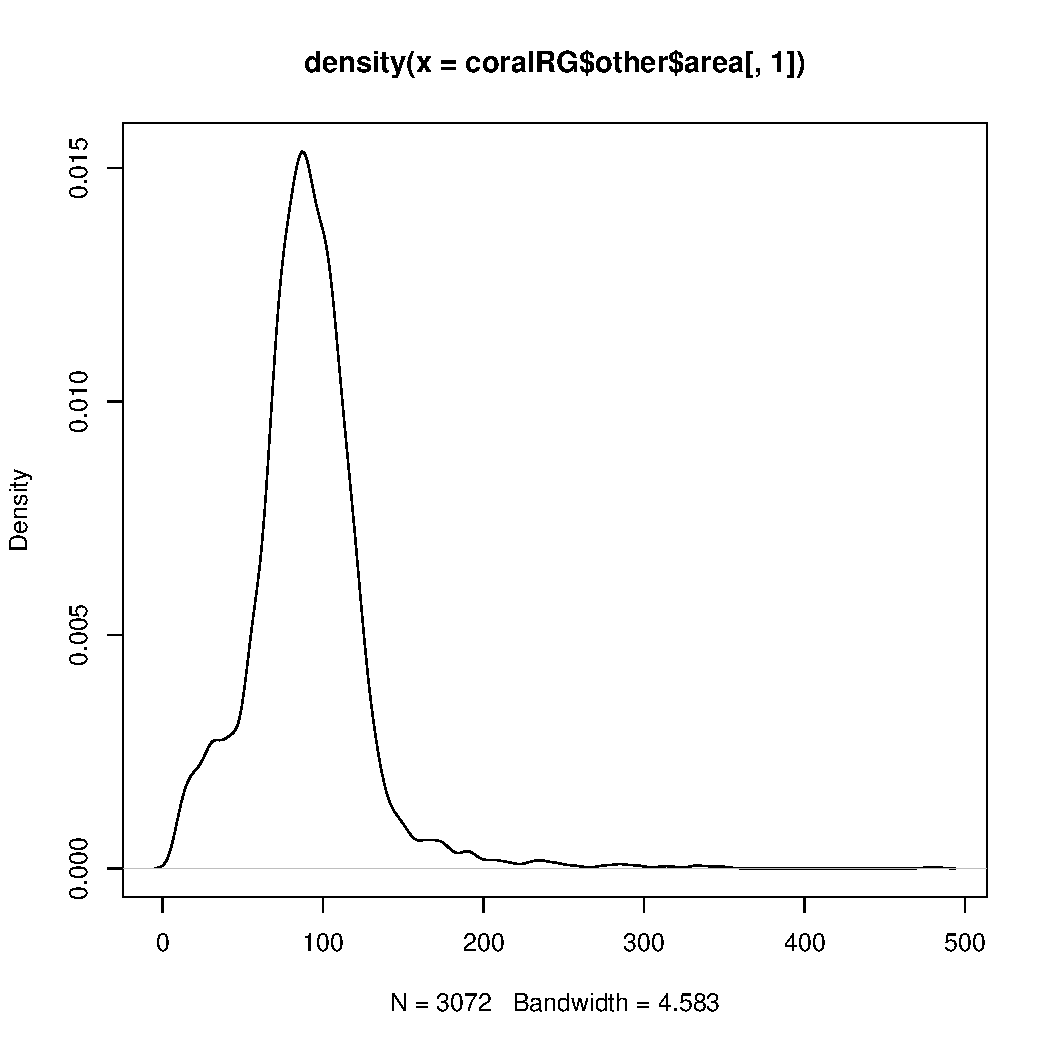
\includegraphics[width=\maxwidth]{figure/unnamed-chunk-2-1} 
\end{knitrout}
The \textit{limma} package does actually allow for the use of area
as a measure of quality, with information from spots that are larger
or smaller than the optimum given a reduced weight in the analysis.

\subsubsection*{Sequence annotation and related information}

Next, additional information will be tagged on to the \texttt{coralRG}
structure, first gene annotation information that is read from the
\textbf{.gal} file, and then information on the way that the
half-slides were printed that can be deduced from the gene annotation file.
\begin{knitrout}
\definecolor{shadecolor}{rgb}{0.969, 0.969, 0.969}\color{fgcolor}\begin{kframe}
\begin{alltt}
\hlstd{coralRG}\hlopt{$}\hlstd{genes} \hlkwb{<-} \hlkwd{readGAL}\hlstd{(}\hlkwc{path}\hlstd{=path2data)}
\hlstd{coralRG}\hlopt{$}\hlstd{printer} \hlkwb{<-} \hlkwd{getLayout}\hlstd{(coralRG}\hlopt{$}\hlstd{genes)}
\hlstd{coralRG}\hlopt{$}\hlstd{printer}
\end{alltt}
\end{kframe}
\end{knitrout}
These half slides were printed in a 4 by 4 layout, corresponding to the
4 by 4 layout of the printhead.  Each tip printed an array of 16 rows
by 12 columns.  To see the order in which the spots were printed,
attach the \textit{DAAGbio} package, and run the function
\texttt{plotprintseq()}, thus:
and enter:
\begin{knitrout}
\definecolor{shadecolor}{rgb}{0.969, 0.969, 0.969}\color{fgcolor}\begin{kframe}
\begin{alltt}
\hlkwd{plotprintseq}\hlstd{()}
\end{alltt}
\end{kframe}
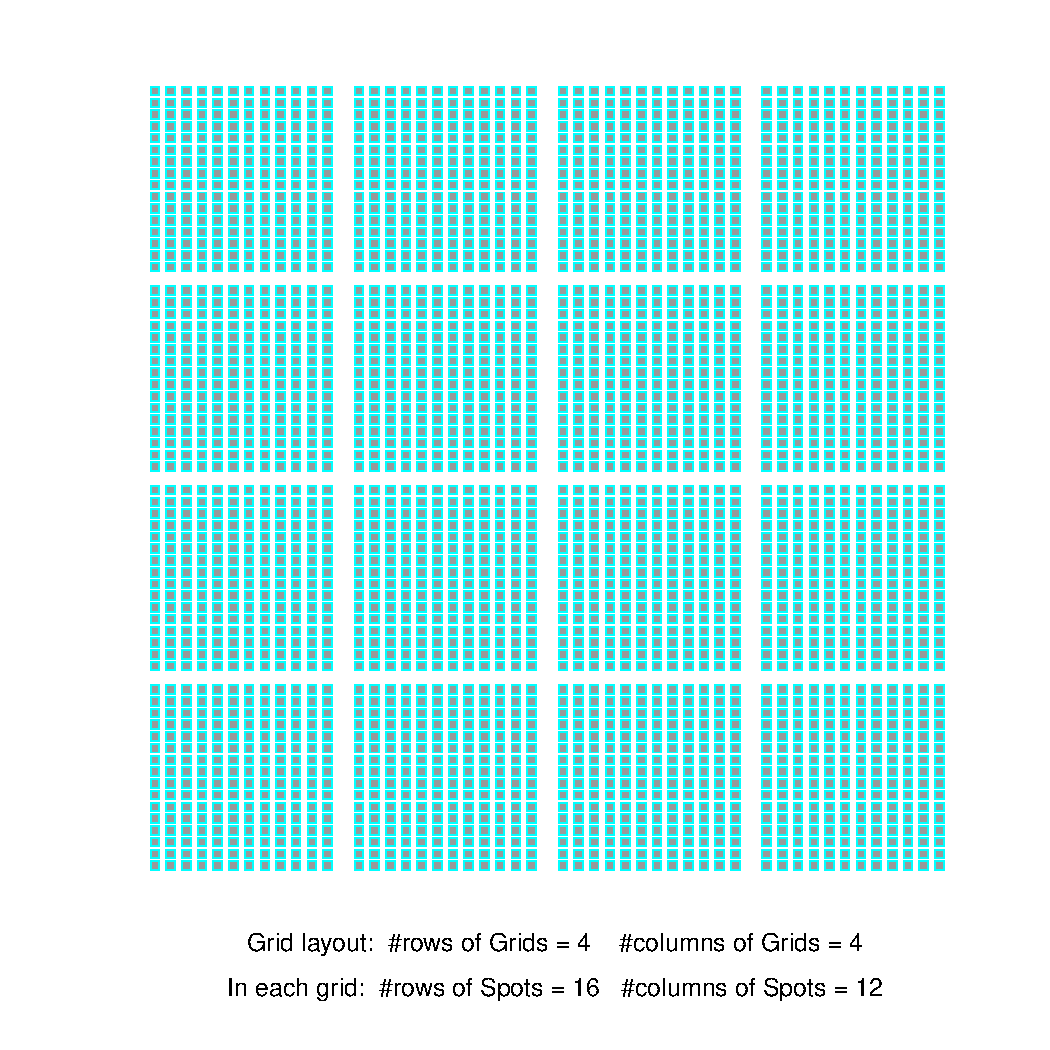
\includegraphics[width=\maxwidth]{figure/printseq-1} 
\end{knitrout}


\subsubsection*{The Spot Types File}
This is optional, but strongly recommended.  Spots can be grouped into
at least four categories -- there are ``genes'' (really, partial gene
sequences), negative controls, blanks and differentially expressed
controls.  Genes may or may not be differentially expressed, the next
three categories should not show evidence of differential expression,
and the differentially expressed controls should mostly show evidence
of differential expression.  Plots that label points according to
their types can be beautiful, insightful and, if they find nothing
amiss, reassuring.

Here is what the file looks like (note that tabs must be
used as separators, for the code below to work without modification):
\begin{verbatim}
SpotType        ID      Name    Color
gene            *       *       black
negative        *       [1-9]*  brown
blank           *       -       yellow
diff-exp ctl    *       DH*     blue
\end{verbatim}
{\noindent \small Any color in the long list given by the function
\texttt{colors()} is acceptable.  Try for example \texttt{royalblue}
or \texttt{hotpink} for calibration spots.  They are much less
effective.  You could use \texttt{coral} in place of \texttt{black}
for the ``gene''!!}

The following extracts the spot type information from the file,
and appends it to the data structure that I have called
\texttt{coralRG}:
\begin{knitrout}
\definecolor{shadecolor}{rgb}{0.969, 0.969, 0.969}\color{fgcolor}\begin{kframe}
\begin{alltt}
\hlstd{spottypes}\hlkwb{<-}\hlkwd{readSpotTypes}\hlstd{(}\hlkwc{path}\hlstd{=path2data)}
\hlstd{coralRG}\hlopt{$}\hlstd{genes}\hlopt{$}\hlstd{Status} \hlkwb{<-} \hlkwd{controlStatus}\hlstd{(spottypes, coralRG)}
\end{alltt}
\begin{verbatim}
## Matching patterns for: ID Name 
## Found 3072 gene 
## Found 7 negative 
## Found 30 blank 
## Found 21 diff-exp ctl 
## Setting attributes: values Color
\end{verbatim}
\end{kframe}
\end{knitrout}

\section{Plots}

\subsection{Spatial Plots}
These plots use colour scales to summarize, on a layout that reflects
the actual layout of the slide, information on the spots.  The idea is
to check for any strong spatial patterns that might indicate some lack
of uniformity that has resulted from the printing (e.g., one print tip
printing differently from the others), or from uneven conditions in
the hybridization chamber.  There may be surface features, perhaps due
to a hair or to the mishandling of one corner of the slide, this may
show up on the plot.

What is finally important is of course the effect on the log-ratios
(the M-values).  Some unevenness in the separate foreground and
background intensities can be tolerated, providing that it leads to
much the same proportional change in both channels.

There are two possibilities -- to use \texttt{imageplot()} from
\textit{limma}, or to use my function \texttt{imgplot()} that is
included in the \textit{DAAGbio} package; see the appendux.  Here are
plots that use \texttt{imageplot()}:
\begin{knitrout}
\definecolor{shadecolor}{rgb}{0.969, 0.969, 0.969}\color{fgcolor}\begin{kframe}
\begin{alltt}
\hlkwd{imageplot}\hlstd{(}\hlkwd{log2}\hlstd{(coralRG}\hlopt{$}\hlstd{Rb[,} \hlnum{1}\hlstd{]}\hlopt{+}\hlnum{1}\hlstd{),} \hlkwc{layout} \hlstd{= coralRG}\hlopt{$}\hlstd{printer,}
          \hlkwc{low}\hlstd{=}\hlstr{"white"}\hlstd{,} \hlkwc{high}\hlstd{=}\hlstr{"red"}\hlstd{)}
\end{alltt}
\end{kframe}
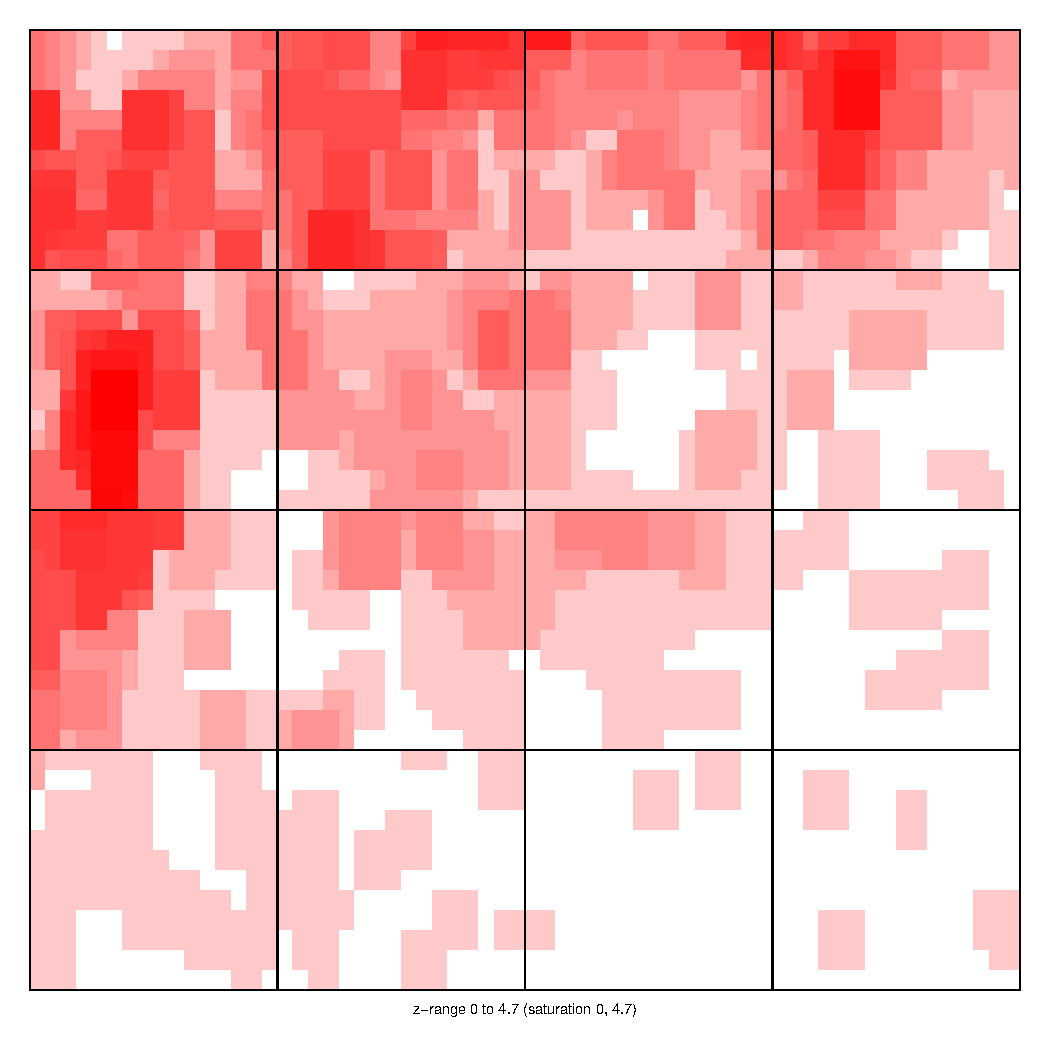
\includegraphics[width=\maxwidth]{figure/unnamed-chunk-5-1} 
\end{knitrout}
This should be repeated for each different half-slide, for both red and
green, and similarly for the green background.  To get the plot for the
second half-slide, type:
\begin{knitrout}
\definecolor{shadecolor}{rgb}{0.969, 0.969, 0.969}\color{fgcolor}\begin{kframe}
\begin{alltt}
\hlkwd{imageplot}\hlstd{(}\hlkwd{log2}\hlstd{(coralRG}\hlopt{$}\hlstd{Rb[,} \hlnum{2}\hlstd{]}\hlopt{+}\hlnum{1}\hlstd{),} \hlkwc{layout} \hlstd{= coralRG}\hlopt{$}\hlstd{printer,}
          \hlkwc{low}\hlstd{=}\hlstr{"white"}\hlstd{,} \hlkwc{high}\hlstd{=}\hlstr{"red"}\hlstd{)}
\end{alltt}
\end{kframe}
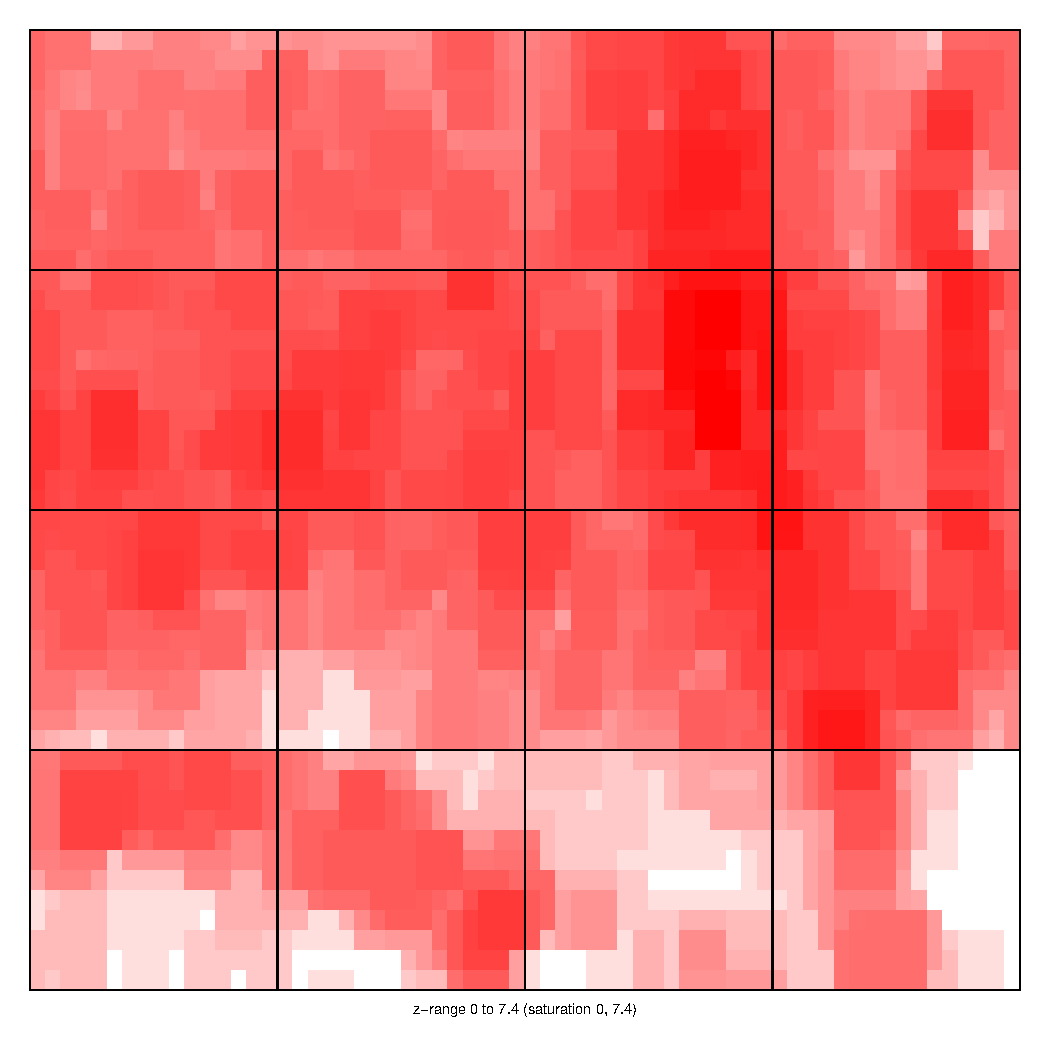
\includegraphics[width=\maxwidth]{figure/unnamed-chunk-6-1} 
\end{knitrout}

The plots can be obtained all six at once, in a three rows by two
columns layout.  For this, use the function \texttt{xplot()},
included in the \textit{DAAGbio} package.

As an example, to get the six plots for the red channel on the screen, type:
\begin{knitrout}
\definecolor{shadecolor}{rgb}{0.969, 0.969, 0.969}\color{fgcolor}\begin{kframe}
\begin{alltt}
\hlkwd{x11}\hlstd{(}\hlkwc{width}\hlstd{=}\hlnum{7.5}\hlstd{,} \hlkwc{height}\hlstd{=}\hlnum{11}\hlstd{)}
\hlkwd{xplot}\hlstd{(}\hlkwc{data} \hlstd{= coralRG}\hlopt{$}\hlstd{R,} \hlkwc{layout} \hlstd{= coralRG}\hlopt{$}\hlstd{printer,} \hlkwc{FUN}\hlstd{=imageplot)}
\end{alltt}
\end{kframe}
\end{knitrout}
(Under Macintosh OSX with the Aqua GUI, specify
\texttt{quartz(width=7.5, height=11)} to use the quartz device.
It is also possible to send the output to a hard copy.  Type, e.g.:
\begin{knitrout}
\definecolor{shadecolor}{rgb}{0.969, 0.969, 0.969}\color{fgcolor}\begin{kframe}
\begin{alltt}
\hlkwd{quartz}\hlstd{(}\hlkwc{width}\hlstd{=}\hlnum{7.5}\hlstd{,} \hlkwc{height}\hlstd{=}\hlnum{11}\hlstd{)}
\hlkwd{xplot}\hlstd{(}\hlkwc{data} \hlstd{= coralRG}\hlopt{$}\hlstd{R,} \hlkwc{layout} \hlstd{= coralRG}\hlopt{$}\hlstd{printer,} \hlkwc{FUN}\hlstd{=imageplot,}
       \hlkwc{device}\hlstd{=pdf)}
\end{alltt}
\end{kframe}
\end{knitrout}
Other possibilities for \texttt{device} are \texttt{device="ps"},
\texttt{device="png"}, \texttt{device="jpeg"} and
\texttt{device="bmp"}.  For \texttt{device="png"} and
\texttt{device="jpeg"} the parameters \texttt{width} and
\texttt{height} will need to be specified, in pixels, in the call to
\texttt{sixplot()}.

\subsection{MA plots \& Normalization}
In this overview, the default background correction will be used, in
which the background is in each case subtracted from the corresponding
measured signal.\footnote{For image files from Spot, this usually
works fairly well.  GenePix gives image files in which the intensities
can be much too high.  There are alternative to subtracting off the
background that may be desirable, perhaps ignoring it altogether.}

At this point normalization is an issue.  The Cy3 channel (``green'')
typically shows up with higher intensity than the Cy5 channel
(``red'').  The measure of differential expression is\[
{\rm M} = \log({\rm red intensity}) - \log({\rm green intensity}) =
\log(\frac{\displaystyle \rm red intensity}
{\displaystyle \rm green intensity})
\]

First, check what happens if we do not normalize.
Try the following:
\begin{knitrout}
\definecolor{shadecolor}{rgb}{0.969, 0.969, 0.969}\color{fgcolor}\begin{kframe}
\begin{alltt}
\hlkwd{plotMA}\hlstd{(coralRG,} \hlkwc{array}\hlstd{=}\hlnum{1}\hlstd{)}
\end{alltt}
\end{kframe}
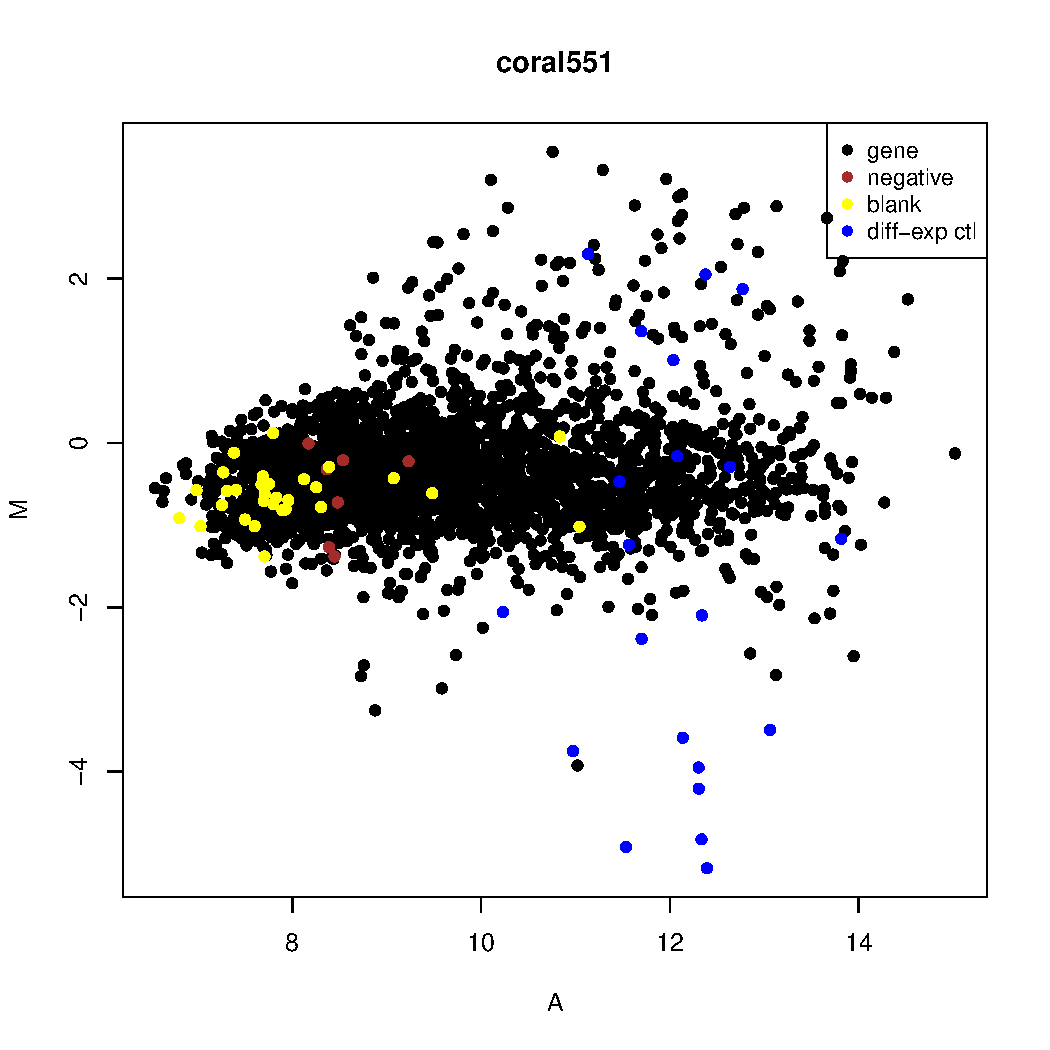
\includegraphics[width=\maxwidth]{figure/unnamed-chunk-7-1} 
\end{knitrout}
This plots the unnormalized log-ratios (the M-values) against the
the averages of the log-intensities for the two separate channels,
i.e., against what are called the A-values.

To see all six arrays in a single plot, precede the six plots
(first with \texttt{array=1}, then \texttt{array=1}, \ldots)
with:
\begin{knitrout}
\definecolor{shadecolor}{rgb}{0.969, 0.969, 0.969}\color{fgcolor}\begin{kframe}
\begin{alltt}
\hlstd{oldpar} \hlkwb{<-} \hlkwd{par}\hlstd{(}\hlkwc{mfrow}\hlstd{=}\hlkwd{c}\hlstd{(}\hlnum{3}\hlstd{,}\hlnum{2}\hlstd{),} \hlkwc{mar}\hlstd{=}\hlkwd{c}\hlstd{(}\hlnum{5.1}\hlstd{,} \hlnum{4.1}\hlstd{,} \hlnum{1.1}\hlstd{,} \hlnum{0.6}\hlstd{))}
\hlcom{## When done with the 3 by 2 layout, be sure to type}
\hlkwd{par}\hlstd{(oldpar)}     \hlcom{# This returns to the original settings.}
\end{alltt}
\end{kframe}
\end{knitrout}
In some of the plots, the dye bias is rather strongly density dependent.

It is also possible to do the following:
\begin{knitrout}
\definecolor{shadecolor}{rgb}{0.969, 0.969, 0.969}\color{fgcolor}\begin{kframe}
\begin{alltt}
\hlstd{rawMA} \hlkwb{<-} \hlkwd{normalizeWithinArrays}\hlstd{(coralRG,} \hlkwc{method} \hlstd{=} \hlstr{"none"}\hlstd{)}
\hlkwd{plotPrintTipLoess}\hlstd{(rawMA,} \hlkwc{array}\hlstd{=}\hlnum{1}\hlstd{)}
\end{alltt}
\end{kframe}
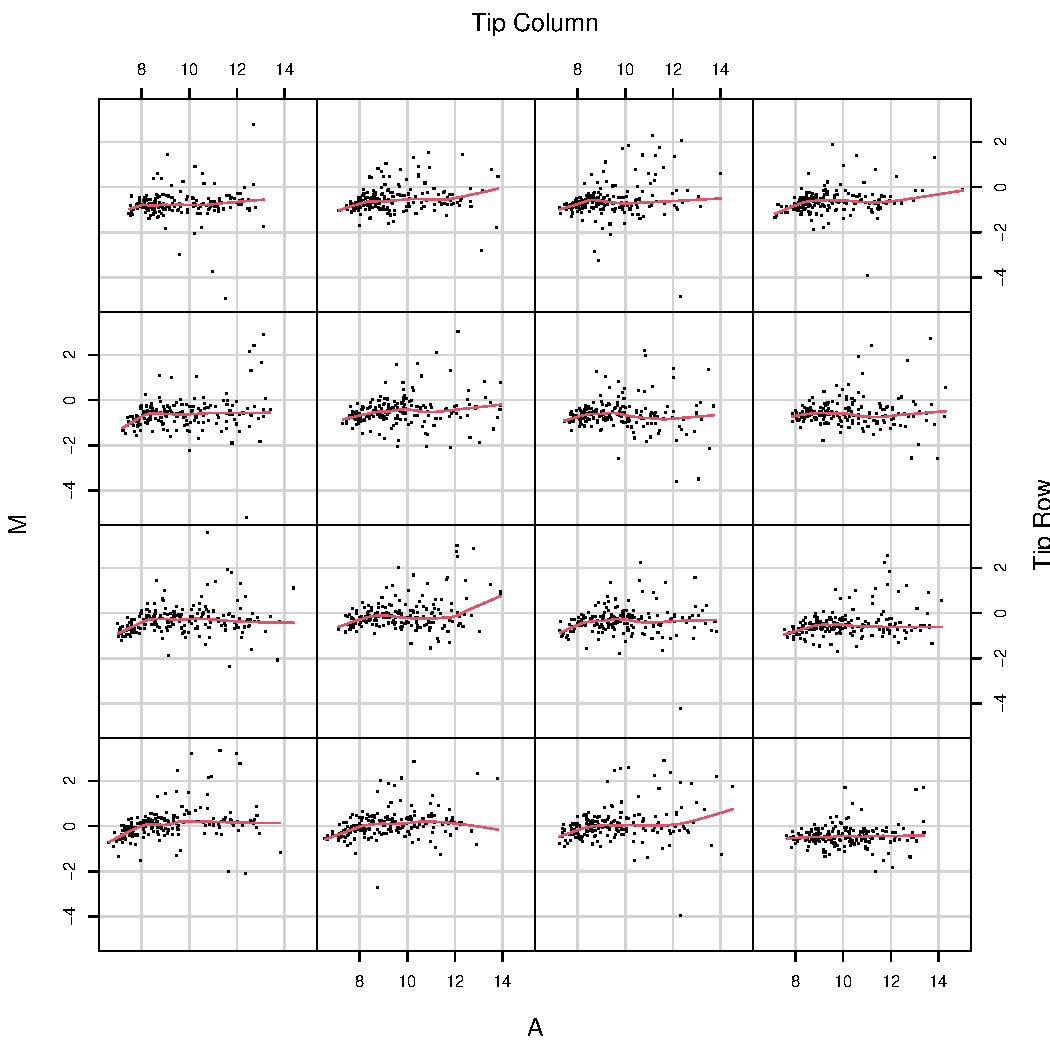
\includegraphics[width=\maxwidth]{figure/unnamed-chunk-8-1} 
\end{knitrout}
A different curve is fitted for each of the print tip groups.
There does seem to be some difference in dye bias between the
different print tip groups.

Next, we apply print tip loess normalization, and check the MA plots:
\begin{knitrout}
\definecolor{shadecolor}{rgb}{0.969, 0.969, 0.969}\color{fgcolor}\begin{kframe}
\begin{alltt}
\hlstd{MA} \hlkwb{<-} \hlkwd{normalizeWithinArrays}\hlstd{(coralRG,} \hlkwc{method} \hlstd{=} \hlstr{"printtiploess"}\hlstd{)}
\hlkwd{plotPrintTipLoess}\hlstd{(MA)}
\end{alltt}
\end{kframe}
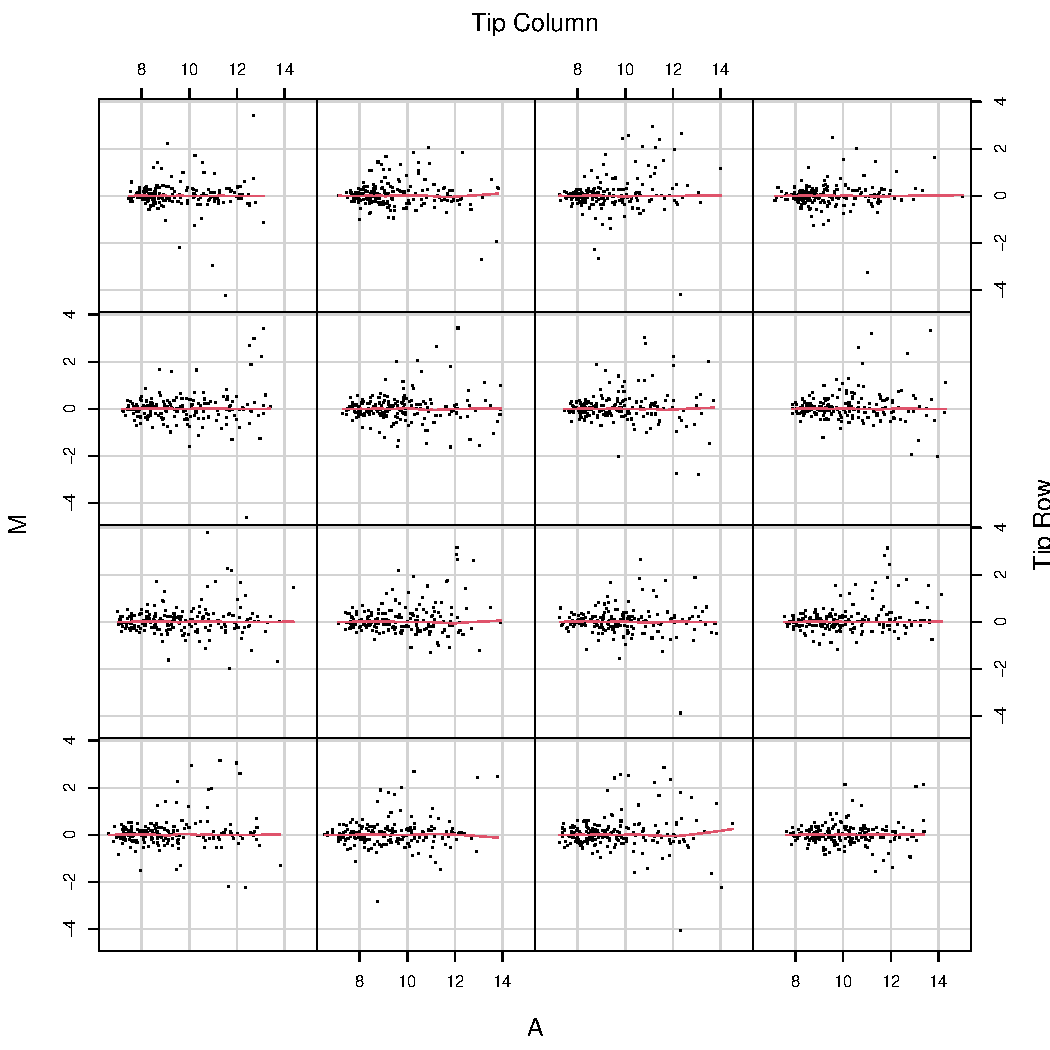
\includegraphics[width=\maxwidth]{figure/unnamed-chunk-9-1} 
\end{knitrout}
Next, we check whether normalization seems required between arrays:
\begin{knitrout}
\definecolor{shadecolor}{rgb}{0.969, 0.969, 0.969}\color{fgcolor}\begin{kframe}
\begin{alltt}
\hlkwd{boxplot}\hlstd{(MA}\hlopt{$}\hlstd{M} \hlopt{~} \hlkwd{col}\hlstd{(MA}\hlopt{$}\hlstd{M),} \hlkwc{names} \hlstd{=} \hlkwd{colnames}\hlstd{(MA}\hlopt{$}\hlstd{M))}
\end{alltt}
\end{kframe}
\end{knitrout}
(There is a helpful explanation of boxplots at:
\url{http://davidmlane.com/hyperstat/A38393.html})

As the arrays seem to have different spreads of M-values, we scale
normalize between arrays, and repeat the boxplot:
\begin{knitrout}
\definecolor{shadecolor}{rgb}{0.969, 0.969, 0.969}\color{fgcolor}\begin{kframe}
\begin{alltt}
\hlstd{nMA} \hlkwb{<-} \hlkwd{normalizeBetweenArrays}\hlstd{(MA)}
\hlkwd{boxplot}\hlstd{(nMA}\hlopt{$}\hlstd{M} \hlopt{~} \hlkwd{col}\hlstd{(nMA}\hlopt{$}\hlstd{M),} \hlkwc{names} \hlstd{=} \hlkwd{colnames}\hlstd{(nMA}\hlopt{$}\hlstd{M))}
\end{alltt}
\end{kframe}
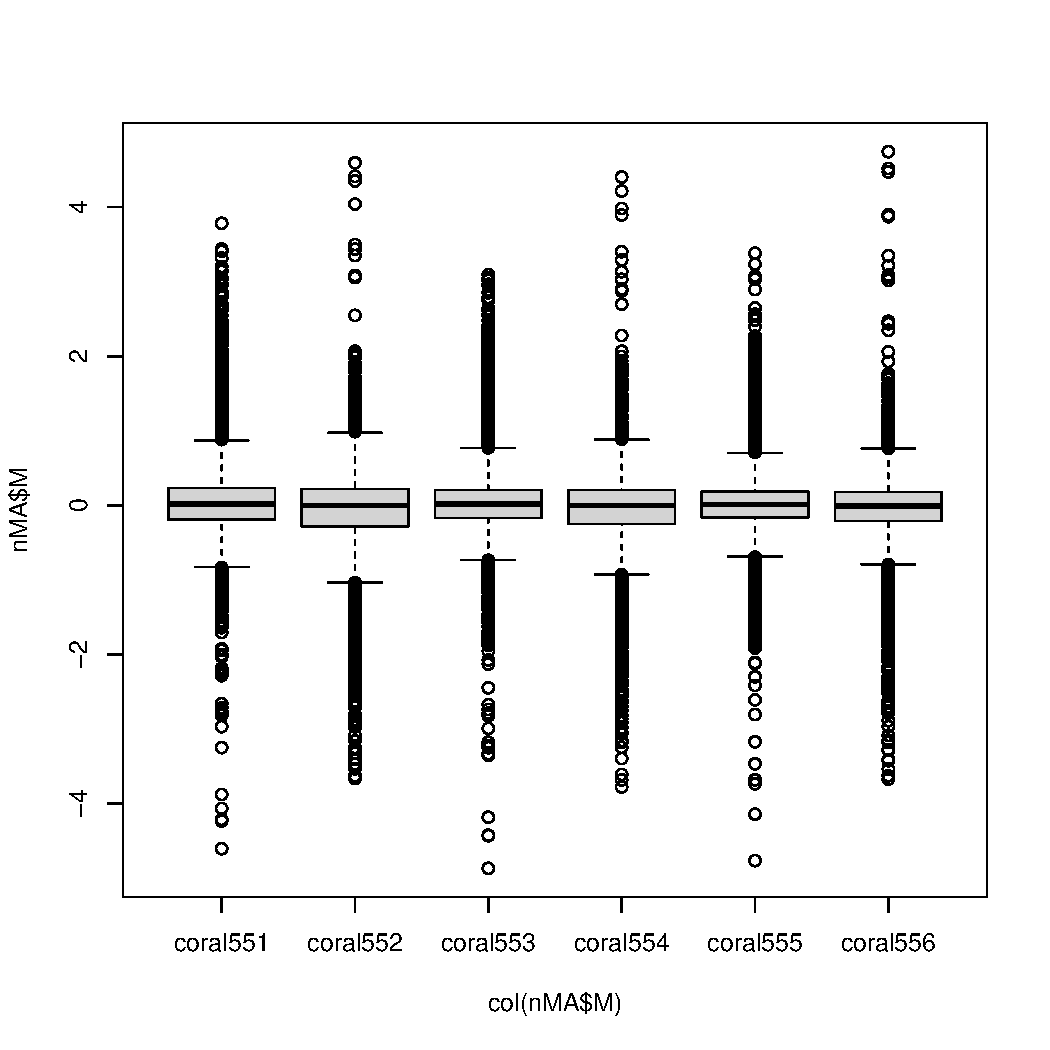
\includegraphics[width=\maxwidth]{figure/unnamed-chunk-11-1} 
\end{knitrout}
The scaling ensures that the medians, and the upper and lower quartiles,
agree across the different slides.

\subsubsection*{Checks on the Differentially Expressed Controls}

The differentially expressed controls ought to show similar evidence of
differential expression on all sets of results. Do they?

We extract the M-values for the differentially expressed controls
from the total data.
\begin{knitrout}
\definecolor{shadecolor}{rgb}{0.969, 0.969, 0.969}\color{fgcolor}\begin{kframe}
\begin{alltt}
\hlstd{wanted} \hlkwb{<-} \hlstd{coralRG}\hlopt{$}\hlstd{genes}\hlopt{$}\hlstd{Status} \hlopt{==} \hlstr{"diff-exp ctl"}
\hlstd{rawdeM} \hlkwb{<-} \hlstd{rawMA}\hlopt{$}\hlstd{M[wanted, ]}
\hlkwd{pairs}\hlstd{(rawdeM)}
\end{alltt}
\end{kframe}
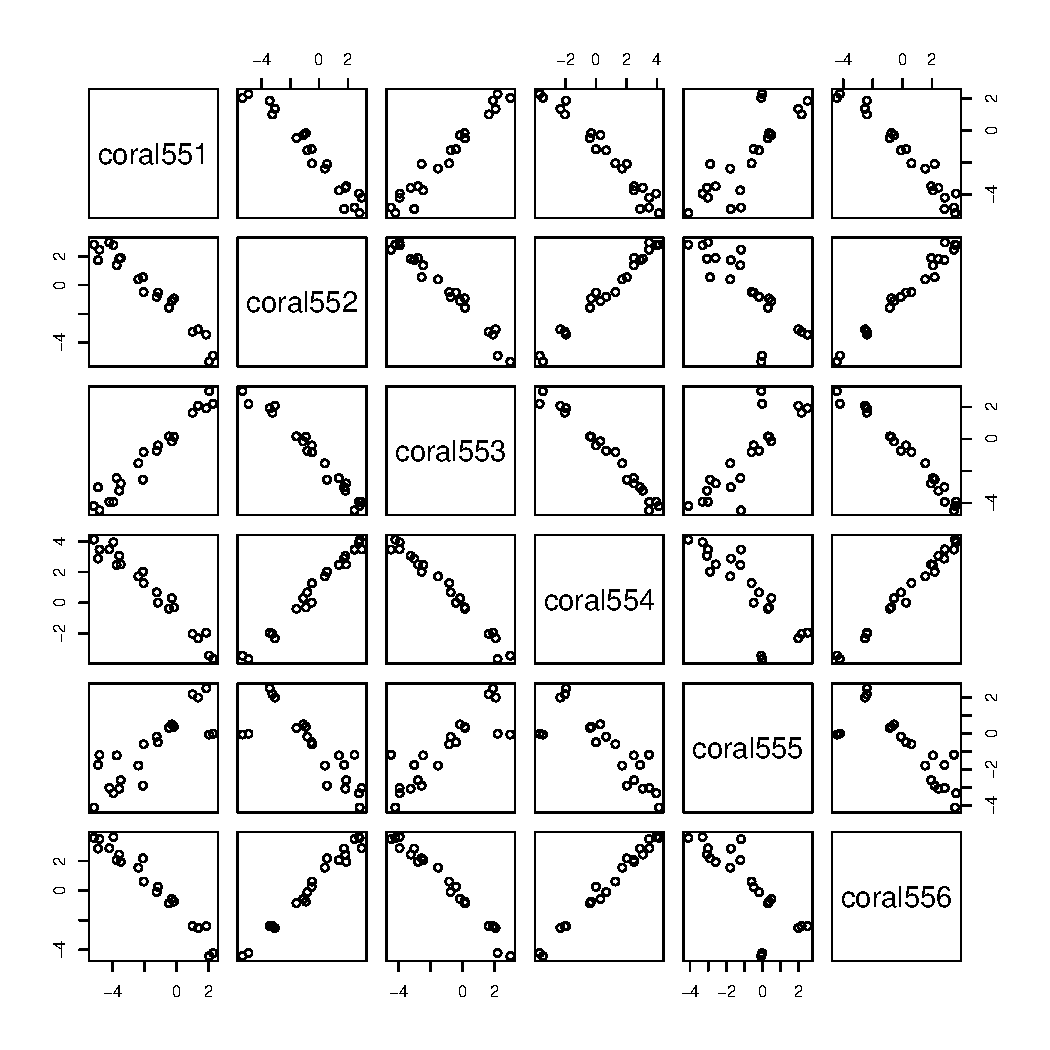
\includegraphics[width=\maxwidth]{figure/unnamed-chunk-12-1} 
\end{knitrout}
The differentially expressed controls line up remarkably well
across the different half-slides.  Notice that half-slide 5 is the odd
one out.  (Why is the correlation sometimes positive and
sometimes negative? What is the pattern?)

We now repeat this exercise with the normalized data:
\begin{knitrout}
\definecolor{shadecolor}{rgb}{0.969, 0.969, 0.969}\color{fgcolor}\begin{kframe}
\begin{alltt}
\hlstd{wanted} \hlkwb{<-} \hlstd{coralRG}\hlopt{$}\hlstd{genes}\hlopt{$}\hlstd{Status} \hlopt{==} \hlstr{"diff-exp ctl"}
\hlstd{deM} \hlkwb{<-} \hlstd{nMA}\hlopt{$}\hlstd{M[wanted, ]}
\hlkwd{pairs}\hlstd{(rawdeM)}
\end{alltt}
\end{kframe}
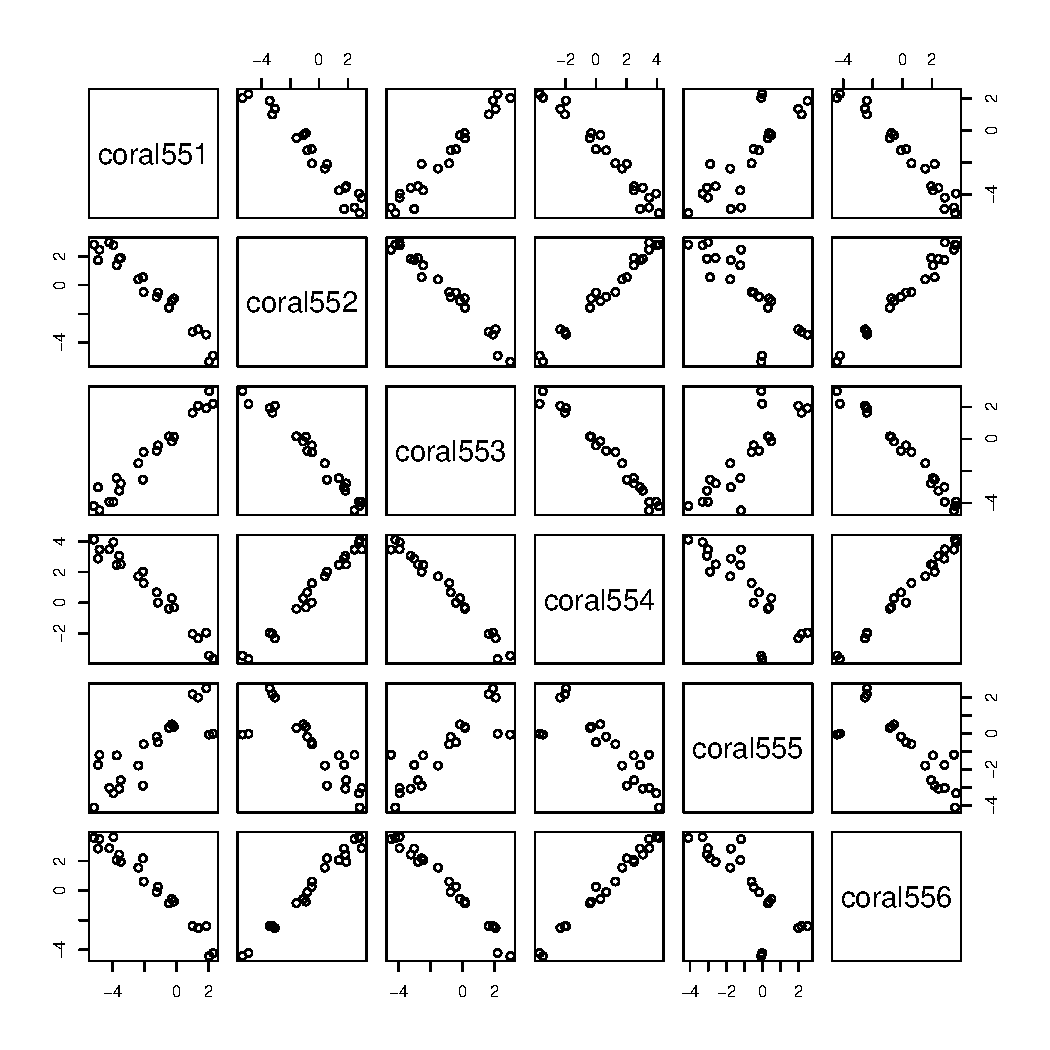
\includegraphics[width=\maxwidth]{figure/unnamed-chunk-13-1} 
\end{knitrout}
Half-slide 5 is still a maverick.  The differentially expressed
controls from the other half-slides line up beautifully.\newline [Dear
me! Every family of more than two or three has a misfit.  We'll banish
half-slide 5 from our assemblage, at least until we can think of
something better to do with it.]

\subsubsection*{More plots}
Use \texttt{imageplot()} with the M-values on all these half-slides, and look
especially at half-slide 5, thus:
\begin{knitrout}
\definecolor{shadecolor}{rgb}{0.969, 0.969, 0.969}\color{fgcolor}\begin{kframe}
\begin{alltt}
\hlkwd{imageplot}\hlstd{(nMA}\hlopt{$}\hlstd{M[,}\hlnum{5}\hlstd{],} \hlkwc{layout}\hlstd{=coralRG}\hlopt{$}\hlstd{printer)}
\end{alltt}
\end{kframe}
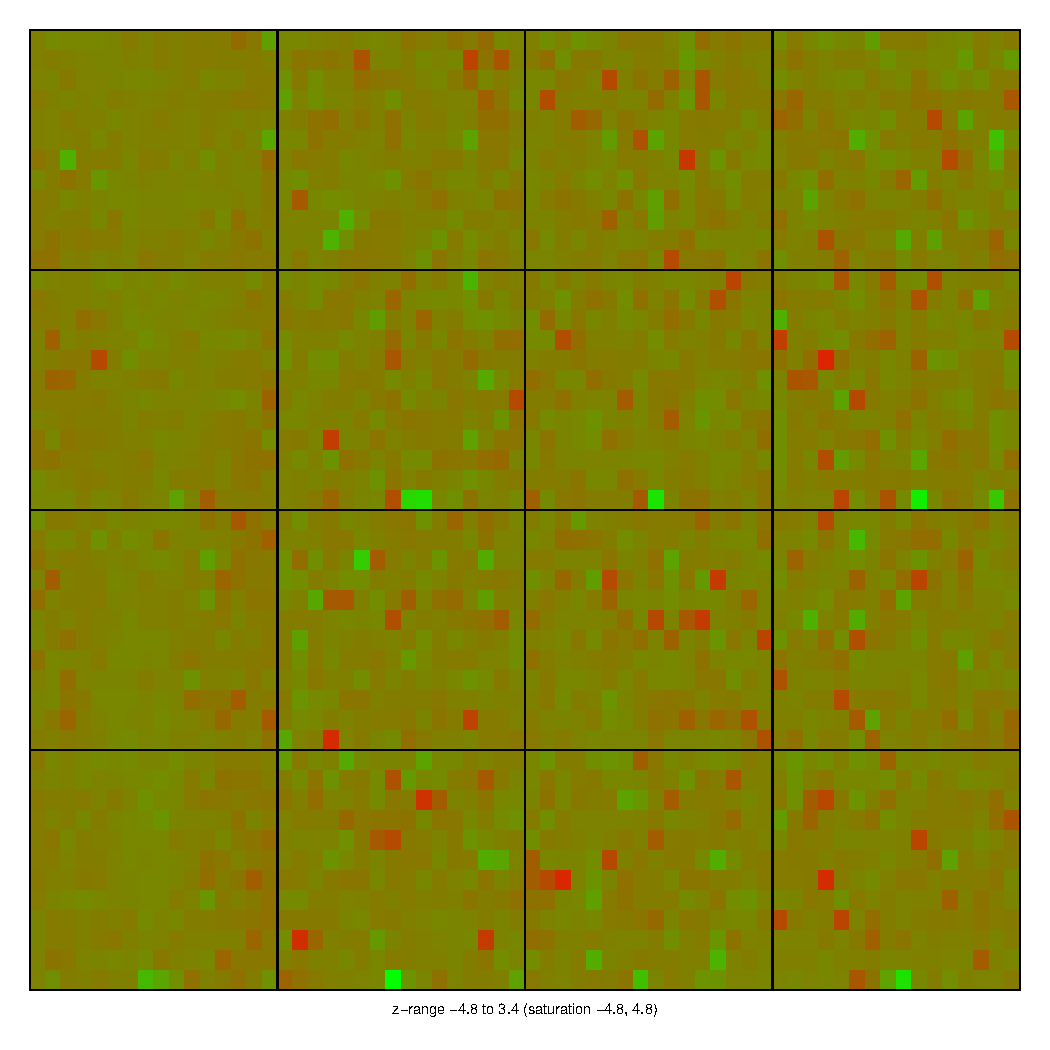
\includegraphics[width=\maxwidth]{figure/unnamed-chunk-14-1} 
\end{knitrout}
Something bad clearly happened to the left side of this half-slide!

\section{Tests for Differential Expression}
We fit a simple statistical model that allows for the possible
effect of the dye swap, and which we can use as the basis for
checks for differential expression.
Recall that ${\rm M} = \log({\rm red intensity}) - \log({\rm green intensity})$.
Here is how this connects with treatments:
\vspace*{3pt}

\begin{tabular}{lcccccc}
Slide & 221a & 221b & 223a & 223b & 224a & 224b \\
\hline
 & $\log({\rm pre/post)}$ & $\log({\rm post/pre)}$
 & $\log({\rm pre/post)}$ & $\log({\rm post/pre)}$
 & $\log({\rm pre/post)}$ & $\log({\rm post/pre)}$ \\
Xply by & -1 & 1 &  -1 & 1 &  0 & 1 \\
\hline
\end{tabular}
\vspace*{3pt}

Results for the first and third half-slide are multiplied by -1,
so that $\log({\rm pre/post)}$ (which equals
$\log({\rm pre}) - \log({\rm post)}$ becomes $\log({\rm post/pre)}$.
The 0 for the fifth half-slide will omit it altogether.
This is achieved by placing these numbers into a ``design vector''.
\begin{knitrout}
\definecolor{shadecolor}{rgb}{0.969, 0.969, 0.969}\color{fgcolor}\begin{kframe}
\begin{alltt}
\hlstd{design} \hlkwb{<-} \hlkwd{c}\hlstd{(}\hlopt{-}\hlnum{1}\hlstd{,} \hlnum{1}\hlstd{,} \hlopt{-}\hlnum{1}\hlstd{,} \hlnum{1}\hlstd{,} \hlnum{0}\hlstd{,} \hlnum{1}\hlstd{)}
\end{alltt}
\end{kframe}
\end{knitrout}

\subsubsection*{Fitting the statistical model}
To fit a model that reflects this design, specify:
\begin{knitrout}
\definecolor{shadecolor}{rgb}{0.969, 0.969, 0.969}\color{fgcolor}\begin{kframe}
\begin{alltt}
\hlstd{fit} \hlkwb{<-} \hlkwd{lmFit}\hlstd{(nMA, design)}
\end{alltt}
\end{kframe}
\end{knitrout}
This basically gives $t$-test results for all the different spots.
Any attempt at interpretation has to take account of the large number
of tests that have been performed.  Also, because there are just 5
sets of usable M-values, the variances that are used in the
denominators of the $t$-statistics, and hence the $t$-statistics
themselves, are more unstable than is desirable.

The calculations that now follow take us into much more speculative
territory, where different software uses different approaches.
My view is that the calculations that are demonstrated are close
to the best that are at present available:  They do three things:
\begin{itemize}
\item They use information from the variances for all spots,
combining this with the spot-specific information, to get
more stable $t$-statistics.
\item They make an adjustment for the multiplicity of tests,
leading to adjusted $t$-statistics that can pretty much be
compared with the usual one-sample $t$-critical values.\newline
[There are many ways to do this.  Also the function requires
a prior estimate of the proportion of genes that are differentially
expressed, by default set to 0.01, i.e.\ there is a large element
of subjective judgment.]
\item For each gene they give an odds ratio ($B$ = Bayes factor) that
      it is differentially expressed.  [This relies on the same prior
      estimate of the proportion of genes that are differentially
      expressed.]
\end{itemize}

From the fit object, we calculate empirical Bayes moderated
$t$-statistics and do a qq-plot:
\begin{knitrout}
\definecolor{shadecolor}{rgb}{0.969, 0.969, 0.969}\color{fgcolor}\begin{kframe}
\begin{alltt}
\hlstd{efit} \hlkwb{<-} \hlkwd{eBayes}\hlstd{(fit)}
\hlkwd{qqt}\hlstd{(efit}\hlopt{$}\hlstd{t,} \hlkwc{df} \hlstd{= efit}\hlopt{$}\hlstd{df.prior} \hlopt{+} \hlstd{efit}\hlopt{$}\hlstd{df.residual,} \hlkwc{pch} \hlstd{=} \hlnum{16}\hlstd{,}
    \hlkwc{cex} \hlstd{=} \hlnum{0.2}\hlstd{)}
\end{alltt}
\end{kframe}
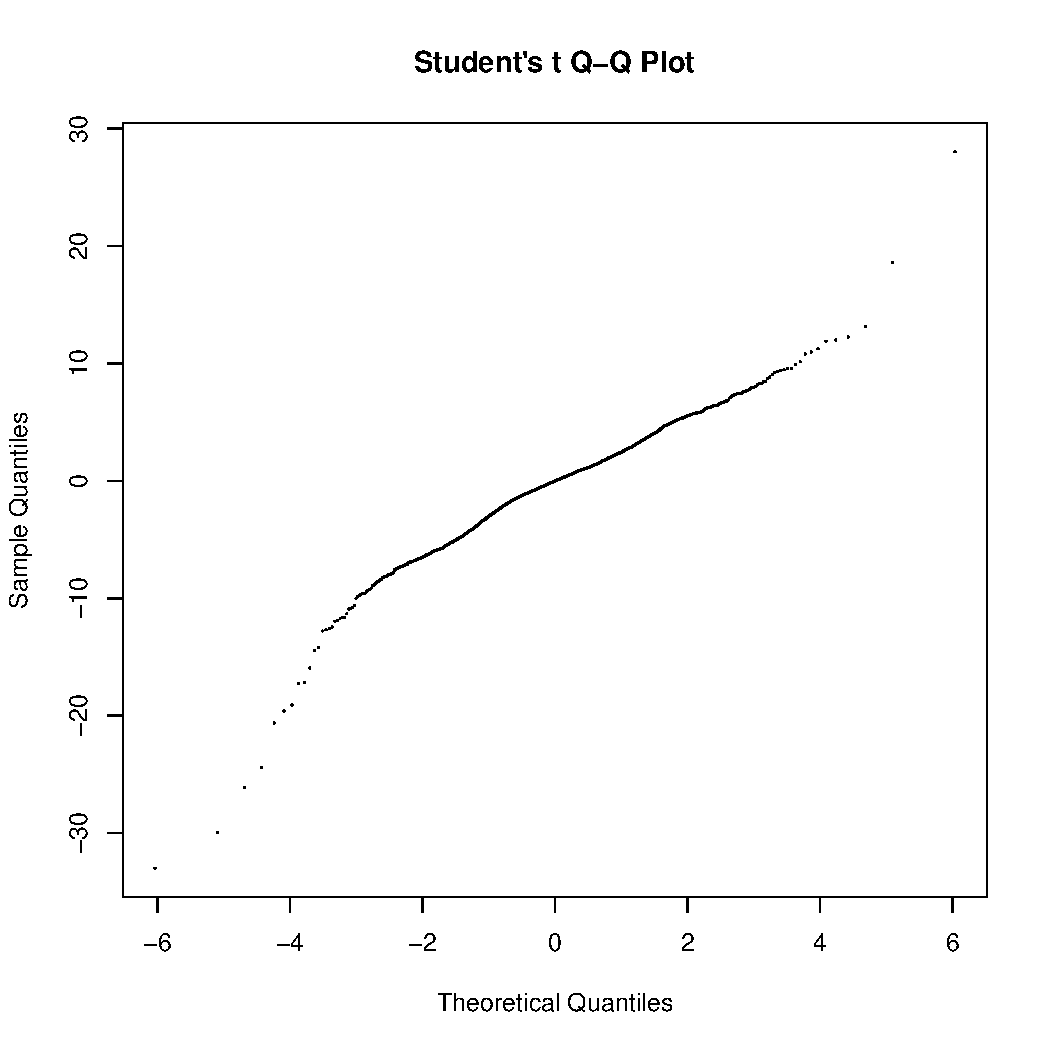
\includegraphics[width=\maxwidth]{figure/unnamed-chunk-17-1} 
\end{knitrout}
The majority of genes lie on a line that goes through the centre of
the plot.  Those that lie off this (below it on the left, or above it
on the right) are most likely to be differentially expressed.
\footnote{If the results from the different genes were independent,
the line on which most of the ``genes'' lie would be a 45$^\circ$
line, with a slope of 1.0.  If you wish, type \texttt{abline(0, 1,
col="red")} to put in such a line anyway. The line on which most of
the genes lie has a much steeper slope than this 45$^\circ$ line.}

Next we print out a table that shows the top 50 differentially
expressed genes, in order of the moderated $t$-statistic values:
\begin{knitrout}
\definecolor{shadecolor}{rgb}{0.969, 0.969, 0.969}\color{fgcolor}\begin{kframe}
\begin{alltt}
\hlkwd{options}\hlstd{(}\hlkwc{digits} \hlstd{=} \hlnum{3}\hlstd{)}
\hlstd{topvals} \hlkwb{<-} \hlkwd{topTable}\hlstd{(efit,} \hlkwc{number} \hlstd{=} \hlnum{50}\hlstd{)}
\hlstd{topvals}
\end{alltt}
\end{kframe}
\end{knitrout}
We store the results in \texttt{topvals} prior to displaying them,
as they will be used later.  Notice that an adjusted $p$-value of 0.05
corresponds to a $B$-statistic of about 3.6.  This may be a reasonably
cut-off point.

The order of genes on the list is much more secure than the $B$-values
and $P$-values.  The extent to which the statistics are affected by the
prior probability will be demonstrated in the exercise below.

Here is another type of plot:
\begin{knitrout}
\definecolor{shadecolor}{rgb}{0.969, 0.969, 0.969}\color{fgcolor}\begin{kframe}
\begin{alltt}
\hlkwd{plot}\hlstd{(efit}\hlopt{$}\hlstd{coef, efit}\hlopt{$}\hlstd{lods,} \hlkwc{pch} \hlstd{=} \hlnum{16}\hlstd{,} \hlkwc{cex} \hlstd{=} \hlnum{0.2}\hlstd{,} \hlkwc{xlab} \hlstd{=} \hlstr{"log(fold change)"}\hlstd{,}
    \hlkwc{ylab} \hlstd{=} \hlstr{"log(odds)"}\hlstd{)}
\hlstd{ord} \hlkwb{<-} \hlkwd{order}\hlstd{(efit}\hlopt{$}\hlstd{lods,} \hlkwc{decreasing} \hlstd{=} \hlnum{TRUE}\hlstd{)}
\hlstd{top8} \hlkwb{<-} \hlstd{ord[}\hlnum{1}\hlopt{:}\hlnum{8}\hlstd{]}
\hlkwd{text}\hlstd{(efit}\hlopt{$}\hlstd{coef[top8], efit}\hlopt{$}\hlstd{lods[top8],} \hlkwc{labels} \hlstd{= coralRG}\hlopt{$}\hlstd{genes[top8,}
    \hlstr{"Name"}\hlstd{],} \hlkwc{cex} \hlstd{=} \hlnum{0.8}\hlstd{,} \hlkwc{col} \hlstd{=} \hlstr{"blue"}\hlstd{)}
\end{alltt}
\end{kframe}
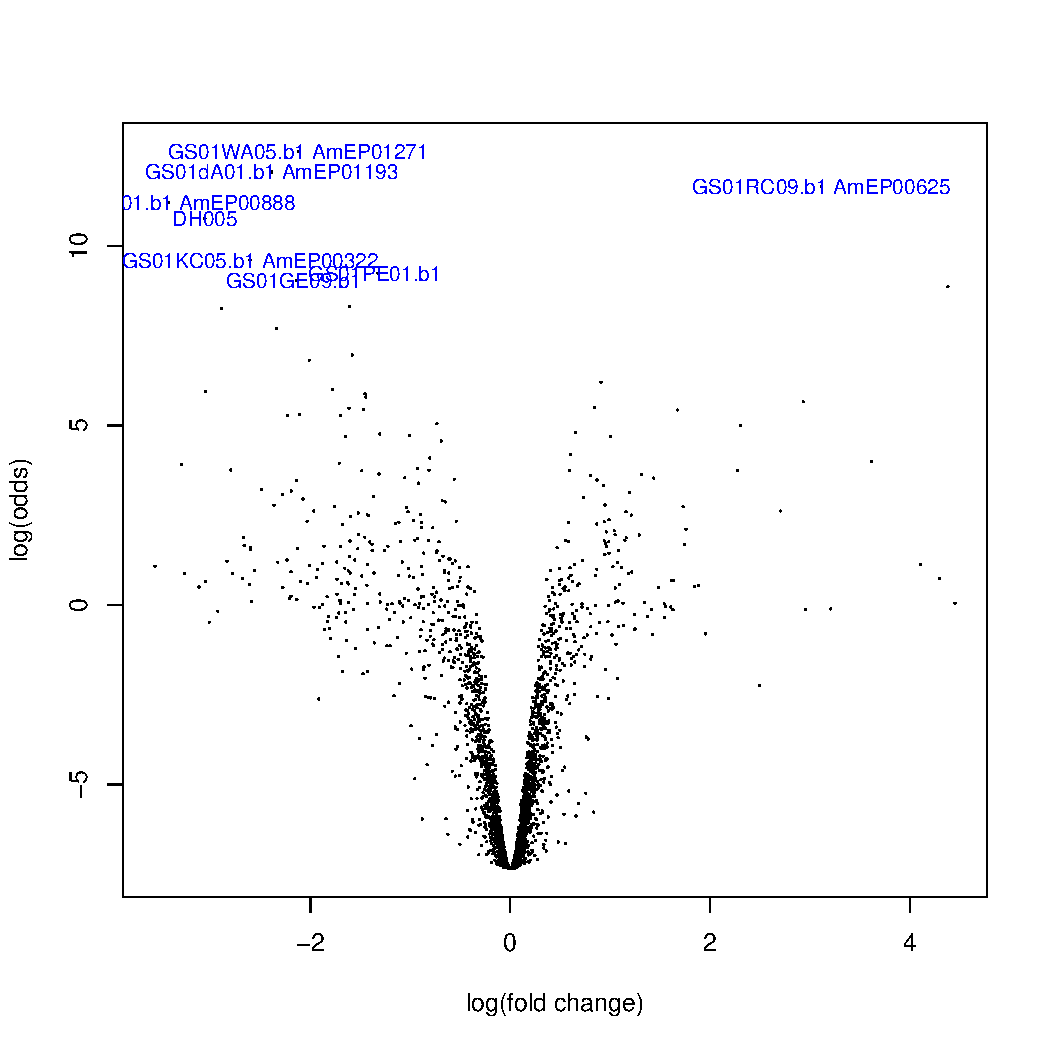
\includegraphics[width=\maxwidth]{figure/unnamed-chunk-19-1} 
\end{knitrout}

\paragraph{Exercise:} Change the prior probability to 0.02, i.e.
\begin{knitrout}
\definecolor{shadecolor}{rgb}{0.969, 0.969, 0.969}\color{fgcolor}\begin{kframe}
\begin{alltt}
\hlstd{efit.02} \hlkwb{<-} \hlkwd{eBayes}\hlstd{(fit,} \hlkwc{prop}\hlstd{=}\hlnum{0.02}\hlstd{)}
\hlkwd{topTable}\hlstd{(efit.02,} \hlkwc{number} \hlstd{=} \hlnum{50}\hlstd{)}
\end{alltt}
\end{kframe}
\end{knitrout}
Observe what difference this makes to the list.  Try also \texttt{prob=0.1}.
A good way to see the effect is to plot the \texttt{P.Value} or \texttt{B}
from the separate fits, one against the other:
\begin{knitrout}
\definecolor{shadecolor}{rgb}{0.969, 0.969, 0.969}\color{fgcolor}\begin{kframe}
\begin{alltt}
\hlstd{efit.1} \hlkwb{<-} \hlkwd{eBayes}\hlstd{(fit,} \hlkwc{prop}\hlstd{=}\hlnum{0.1}\hlstd{)}
\hlstd{B.1} \hlkwb{<-} \hlkwd{topTable}\hlstd{(efit.1,} \hlkwc{number} \hlstd{=} \hlnum{3072}\hlstd{)}\hlopt{$}\hlstd{B}
\hlstd{B.01} \hlkwb{<-} \hlstd{topvals}\hlopt{$}\hlstd{B}
\hlkwd{points}\hlstd{(B.01, B.1,} \hlkwc{col}\hlstd{=}\hlstr{"gray"}\hlstd{)}
\end{alltt}
\end{kframe}
\end{knitrout}

Do the equivalent plots for \texttt{P.Value}.

\section{More refined analyses}
\subsection{Reading Data into R, with weight information incorporated}

Read the data in, with weighting information included:
\begin{knitrout}
\definecolor{shadecolor}{rgb}{0.969, 0.969, 0.969}\color{fgcolor}\begin{kframe}
\begin{alltt}
\hlstd{coral2RG} \hlkwb{<-} \hlkwd{read.maimages}\hlstd{(targets}\hlopt{$}\hlstd{FileName,}
                         \hlkwc{source} \hlstd{=} \hlstr{"spot"}\hlstd{,}
                         \hlkwc{path}\hlstd{=path2data,}
                         \hlkwc{wt.fun}\hlstd{=}\hlkwd{wtarea}\hlstd{(}\hlnum{100}\hlstd{))}
\hlstd{coral2RG}\hlopt{$}\hlstd{genes} \hlkwb{<-} \hlkwd{readGAL}\hlstd{(}\hlkwc{path}\hlstd{=path2data)}
\hlstd{coral2RG}\hlopt{$}\hlstd{printer} \hlkwb{<-} \hlkwd{getLayout}\hlstd{(coral2RG}\hlopt{$}\hlstd{genes)}
\end{alltt}
\end{kframe}
\end{knitrout}
The weights will be used automatically by functions that operate
on \texttt{coral2RG}.

\subsection{MA plots \& Normalization}
Apply print tip loess normalization, and check the MA plots:
\begin{knitrout}
\definecolor{shadecolor}{rgb}{0.969, 0.969, 0.969}\color{fgcolor}\begin{kframe}
\begin{alltt}
\hlstd{MA2} \hlkwb{<-} \hlkwd{normalizeWithinArrays}\hlstd{(coral2RG,} \hlkwc{method} \hlstd{=} \hlstr{"printtiploess"}\hlstd{)}
\hlkwd{plotPrintTipLoess}\hlstd{(MA2)}
\end{alltt}
\end{kframe}
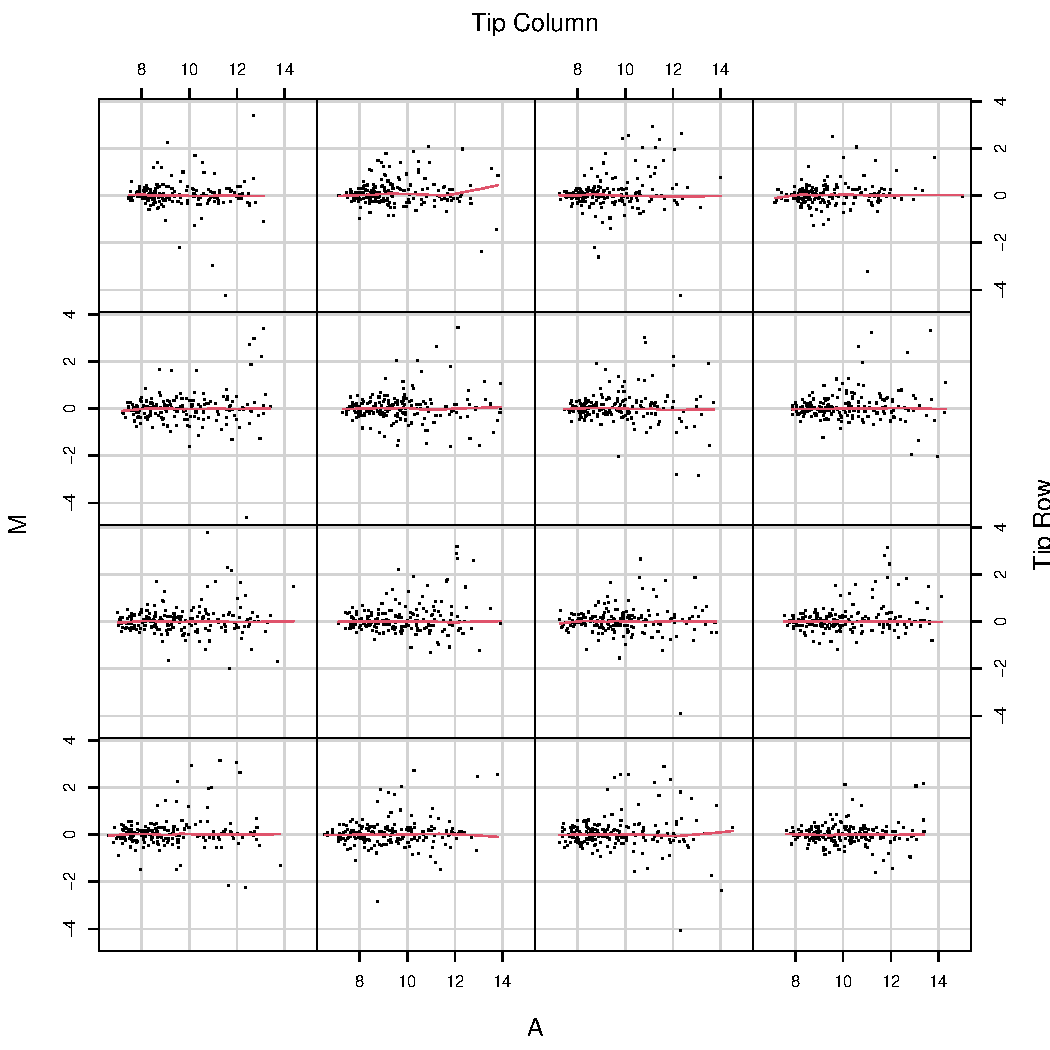
\includegraphics[width=\maxwidth]{figure/unnamed-chunk-21-1} 
\end{knitrout}
Next, we check whether normalization seems required between arrays,
then scale normalize between arrays, and repeat the boxplot:
\begin{knitrout}
\definecolor{shadecolor}{rgb}{0.969, 0.969, 0.969}\color{fgcolor}\begin{kframe}
\begin{alltt}
\hlkwd{boxplot}\hlstd{(MA2}\hlopt{$}\hlstd{M} \hlopt{~} \hlkwd{col}\hlstd{(MA2}\hlopt{$}\hlstd{M),} \hlkwc{names} \hlstd{=} \hlkwd{colnames}\hlstd{(MA2}\hlopt{$}\hlstd{M))}
\end{alltt}
\end{kframe}
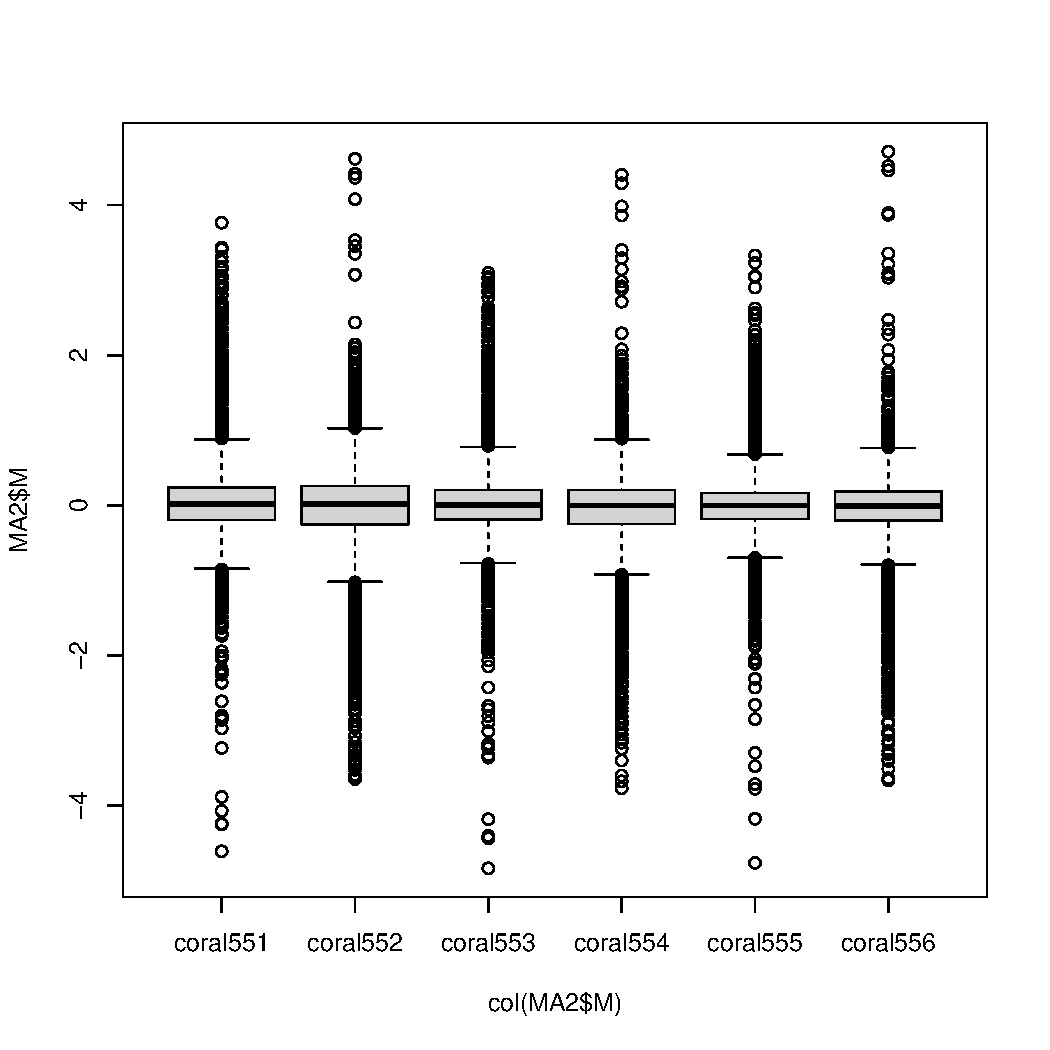
\includegraphics[width=\maxwidth]{figure/unnamed-chunk-22-1} 
\begin{kframe}\begin{alltt}
\hlstd{nMA2} \hlkwb{<-} \hlkwd{normalizeBetweenArrays}\hlstd{(MA2)}
\hlkwd{boxplot}\hlstd{(nMA2}\hlopt{$}\hlstd{M} \hlopt{~} \hlkwd{col}\hlstd{(nMA2}\hlopt{$}\hlstd{M),} \hlkwc{names} \hlstd{=} \hlkwd{colnames}\hlstd{(nMA2}\hlopt{$}\hlstd{M))}
\end{alltt}
\end{kframe}
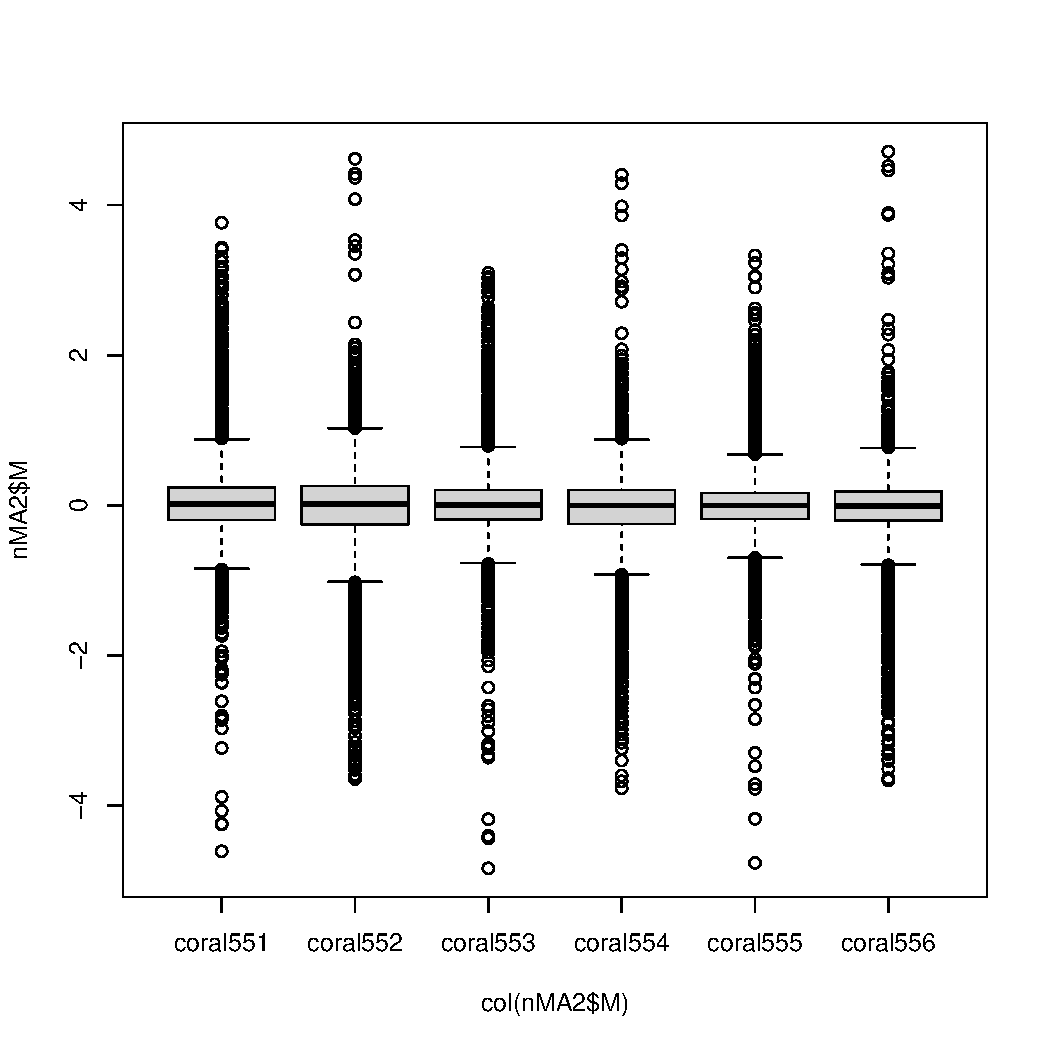
\includegraphics[width=\maxwidth]{figure/unnamed-chunk-22-2} 
\end{knitrout}

\subsubsection*{Slide 5, again!}
Use \texttt{imageplot()} with the M-values on all these half-slides, and look
especially at half-slide 5, thus:
\begin{knitrout}
\definecolor{shadecolor}{rgb}{0.969, 0.969, 0.969}\color{fgcolor}\begin{kframe}
\begin{alltt}
\hlkwd{imageplot}\hlstd{(nMA2}\hlopt{$}\hlstd{M[,}\hlnum{5}\hlstd{],} \hlkwc{layout}\hlstd{=coral2RG}\hlopt{$}\hlstd{printer)}
\end{alltt}
\end{kframe}
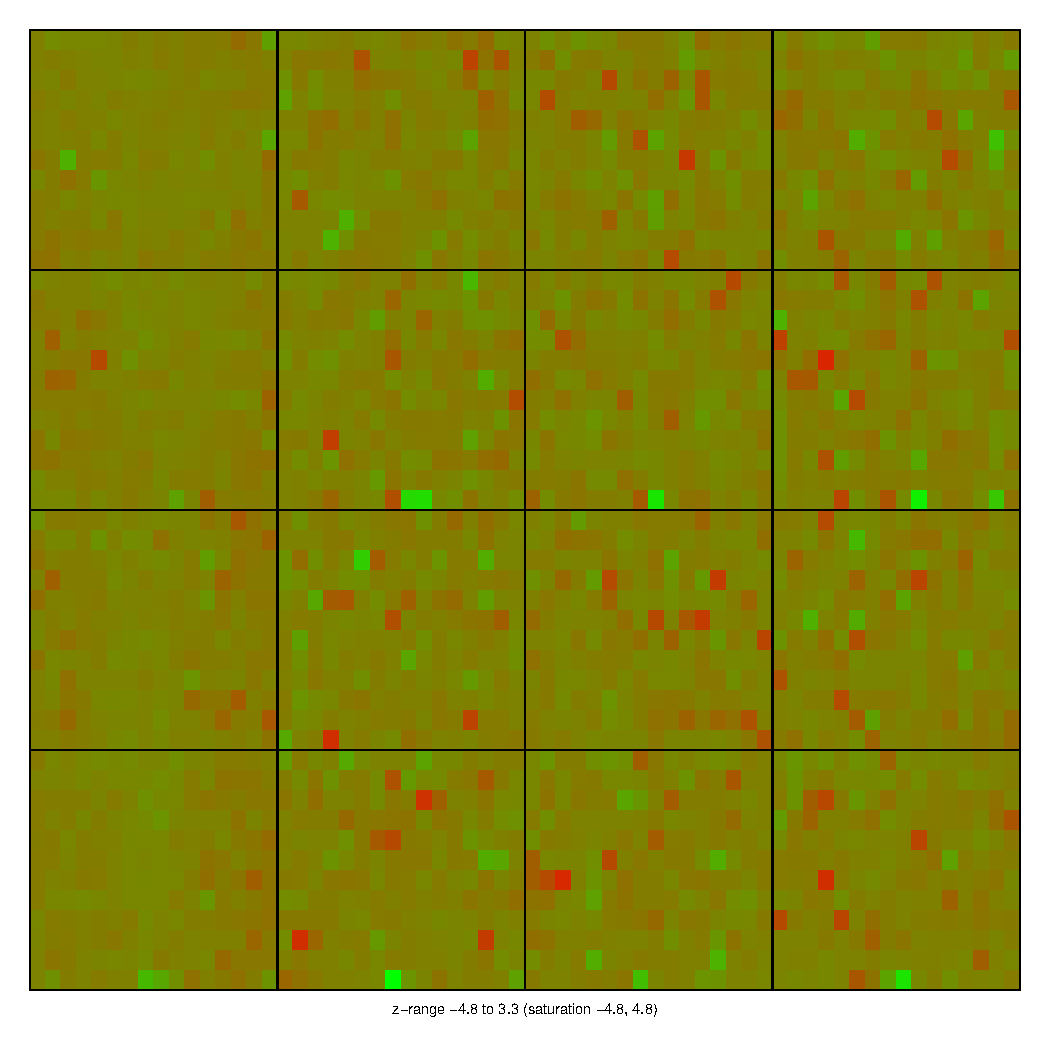
\includegraphics[width=\maxwidth]{figure/unnamed-chunk-23-1} 
\end{knitrout}
Use of the quality information has not made much difference to this plot:

\subsubsection*{Fitting the statistical model}
To fit a model that reflects this design, specify:
\begin{knitrout}
\definecolor{shadecolor}{rgb}{0.969, 0.969, 0.969}\color{fgcolor}\begin{kframe}
\begin{alltt}
\hlstd{design} \hlkwb{<-} \hlkwd{c}\hlstd{(}\hlopt{-}\hlnum{1}\hlstd{,} \hlnum{1}\hlstd{,} \hlopt{-}\hlnum{1}\hlstd{,} \hlnum{1}\hlstd{,} \hlnum{0}\hlstd{,} \hlnum{1}\hlstd{)}
\hlstd{fit2} \hlkwb{<-} \hlkwd{lmFit}\hlstd{(nMA2, design)}
\end{alltt}
\end{kframe}
\end{knitrout}

From the fit object, we calculate empirical Bayes moderated
$t$-statistics and do a qq-plot:
\begin{knitrout}
\definecolor{shadecolor}{rgb}{0.969, 0.969, 0.969}\color{fgcolor}\begin{kframe}
\begin{alltt}
\hlstd{efit2} \hlkwb{<-} \hlkwd{eBayes}\hlstd{(fit2)}
\hlkwd{qqt}\hlstd{(efit2}\hlopt{$}\hlstd{t,} \hlkwc{df} \hlstd{= efit2}\hlopt{$}\hlstd{df.prior} \hlopt{+} \hlstd{efit2}\hlopt{$}\hlstd{df.residual,} \hlkwc{pch} \hlstd{=} \hlnum{16}\hlstd{,}
    \hlkwc{cex} \hlstd{=} \hlnum{0.2}\hlstd{)}
\end{alltt}
\end{kframe}
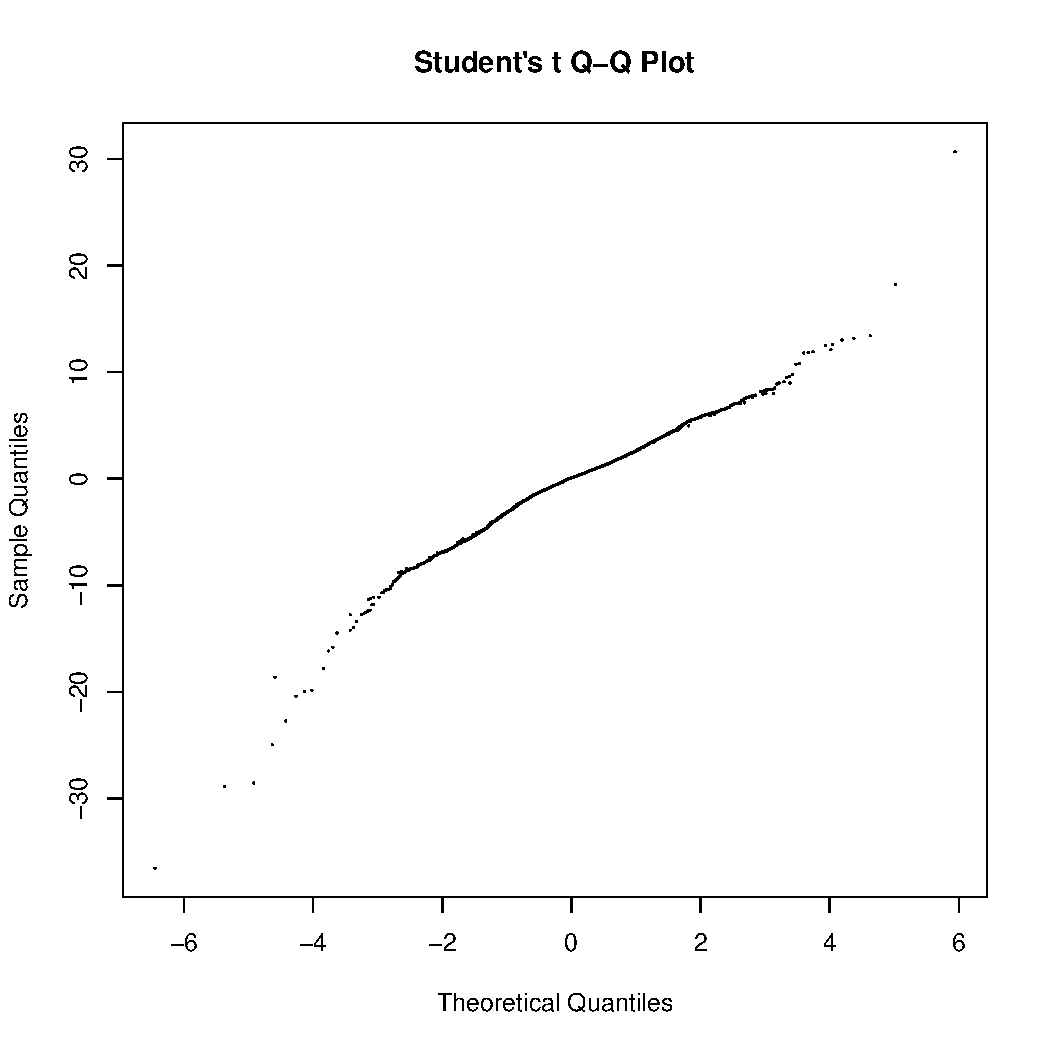
\includegraphics[width=\maxwidth]{figure/unnamed-chunk-25-1} 
\end{knitrout}

Next we print out a table that shows the top 50 differentially
expressed genes, in order of the moderated $t$-statistic values:
\begin{knitrout}
\definecolor{shadecolor}{rgb}{0.969, 0.969, 0.969}\color{fgcolor}\begin{kframe}
\begin{alltt}
\hlkwd{options}\hlstd{(}\hlkwc{digits} \hlstd{=} \hlnum{3}\hlstd{)}
\hlkwd{topTable}\hlstd{(efit2,} \hlkwc{number} \hlstd{=} \hlnum{50}\hlstd{)}
\end{alltt}
\end{kframe}
\end{knitrout}

Now see what different the use of weights has made to the list
(the vector \texttt{topvals} was found earlier):
\begin{knitrout}
\definecolor{shadecolor}{rgb}{0.969, 0.969, 0.969}\color{fgcolor}\begin{kframe}
\begin{alltt}
\hlcom{## Get & store results with & without weights}
\hlstd{topvals2} \hlkwb{<-} \hlkwd{topTable}\hlstd{(efit2,} \hlkwc{number} \hlstd{=} \hlnum{50}\hlstd{)}
\hlkwd{cbind}\hlstd{(}\hlkwd{row.names}\hlstd{(topvals),} \hlkwd{row.names}\hlstd{(topvals2))}
\end{alltt}
\end{kframe}
\end{knitrout}
Now check how many of the genes are in common across both lists:
\begin{knitrout}
\definecolor{shadecolor}{rgb}{0.969, 0.969, 0.969}\color{fgcolor}\begin{kframe}
\begin{alltt}
\hlkwd{sum}\hlstd{(}\hlkwd{row.names}\hlstd{(topvals)}\hlopt\hlkwd{row.names}\hlstd{(topvals2))}
\end{alltt}
\end{kframe}
\end{knitrout}
\section*{Appendix}

\subsection*{Installation of the R software}
First install R (2.10.0 or later).  (Versions are available for Unix,
Linux, Windows and Macintosh OS X.)

Install the \textit{limma} and \textit{DAAGbio} packages.
Install {\em DAAGbio} package from CRAN.  

See \url{http://www.bioconductor.org/packages/release/bioc/html/limma.html}
for instructions on installing {\em limma}. 


\subsection{\texttt{imgplot()} as an alternative to
\texttt{imageplot()}}

The function \texttt{imgplot()} gives a display that is a bit
different from \texttt{imageplot()}. Try:
\begin{knitrout}
\definecolor{shadecolor}{rgb}{0.969, 0.969, 0.969}\color{fgcolor}\begin{kframe}
\begin{alltt}
\hlkwd{imgplot}\hlstd{(coralRG}\hlopt{$}\hlstd{R[,} \hlnum{1}\hlstd{],} \hlkwc{layout} \hlstd{= coralRG}\hlopt{$}\hlstd{printer)}
\end{alltt}
\end{kframe}
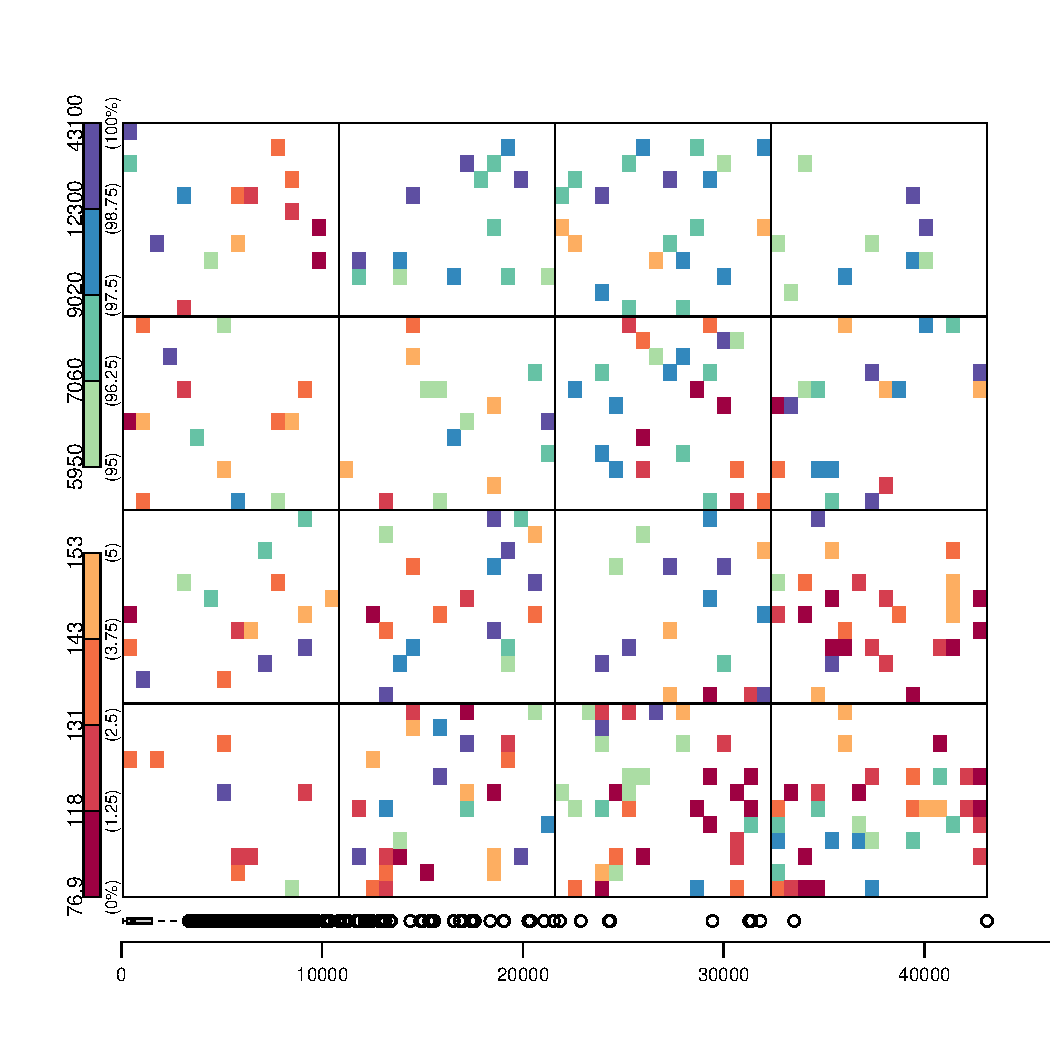
\includegraphics[width=\maxwidth]{figure/unnamed-chunk-29-1} 
\end{knitrout}
By default, this shows just the smallest 5\% of intensities and the
largest 5\% of intensities.

Use these to look for parts of the half-slide that all show a
consistent difference from the rest of the half-slide.
Remember however that what is important is the pattern
that appears after background correction (if any),
normalization and the calculation of the M-values.

\subsection*{How was this document produced?}
The document \textbf{marray-notes.Rnw} can be copied into the
working directory.  

Alternatively, from within an R session, enter:
\begin{knitrout}
\definecolor{shadecolor}{rgb}{0.969, 0.969, 0.969}\color{fgcolor}\begin{kframe}
\begin{alltt}
\hlkwd{library}\hlstd{(knitr)}
\hlkwd{knit}\hlstd{(}\hlstr{"marray-notes.Rnw"}\hlstd{)}
\end{alltt}
\end{kframe}
\end{knitrout}
This produces a \LaTeX\ document that can then be processed through the
\LaTeX\ document preparation system to give a postscript or pdf file.

This is a great way to document your eventual analyses.  Changes to
the code in the \textbf{.Rnw} document are automatically reflected
in the \LaTeX\ document that comes from \texttt{knit()}.
See \texttt{help(knit)} for information on documentation.

\subsection*{References}
\begin{itemize}
\item[] Smythe, G., Thorne, T., and Wettenhall, J. 2004. limma: Linear
Models for Microarray Data User's Guide.  This document is included
with \textit{limma} distributions.
\item[] Beare, R.\ and Buckley, M. 2004. Spot:cDNA Microarray Image
Analysis Users Guide.
Available from \url{http://spot.cmis.csiro.au/spot/spotmanual.php}.
\end{itemize}

\subsection*{Acknowledgements}
Many thanks to Gaby Samuels, Eldon Ball, David Hayward and Rob Saint
(Centre for Molecular Genetics of Development) for permission to use
the coral data for this workshop.  The associated research was
supported by ARC grants DP0343727 (John Maindonald), S4116004
(Lauretta Grasso, Gaby Samuels, Eldon Ball, David Hayward and Rob
Saint, through CMGD).  Conrad Burden did a marvelous job of checking
these notes for mistakes.
\end{document}
